\documentclass[11pt]{article} 
\usepackage[margin=1in]{geometry} 
\usepackage{amsfonts,amsmath,amssymb,graphicx,color}
\usepackage{mathtools}
\usepackage{psfrag} 
\usepackage{pdflscape} 
\usepackage{soul} 
\usepackage{algorithm} 
\usepackage{algpseudocode} 
\usepackage{hyperref} 
\usepackage{multirow} 
\usepackage{caption} 
\usepackage{subcaption}  
% \usepackage{showlabels}
\usepackage{appendix}
\usepackage[T1]{fontenc} 
\usepackage{booktabs} 
\usepackage[normalem]{ulem}
\usepackage{amsthm,hyperre f,fullpage}
\usepackage{float}


\newtheorem{thm}{Theorem}
\newtheorem{lem}[thm]{Lemma}
\newtheorem{cor}[thm]{Corollary}
\newtheorem{rem}[thm]{Remark}

\newcommand{\defeq}{\stackrel{\rm def}{=}}
\newcommand{\defeqq}{\vcentcolon=}
\newcommand{\Var}{\mathrm{Var}}
\newcommand{\E}{\mathbf{E}}

\renewcommand{\theequation}{\thesection.\arabic{equation}}
\newcommand{\comment}[1]{}

\setcounter{section}{0}%


\title{An Evolving Gradient Resampling Method for Stochastic Optimization}

\author{Richard H. Byrd 
\thanks{Department of Computer Science, University of Colorado, Boulder, CO, USA. This author was supported by National Science Foundation grant DMS-1216554 and Department of Energy grant DE-SC0001774.} 
\and Jorge Nocedal 
\thanks{Department of Industrial Engineering and Management Sciences, Northwestern University, Evanston, IL, USA. This author was supported by National Science Foundation grant DMS-0810213, and by Department of Energy grant DE-FG02-87ER25047.} 
\and Figen Oztoprak 
\thanks{Istanbul Technical University. This author was supported by Department of Energy grant DE-SC0001774, and by a grant from Tubitak.} 
\and Stefan Solntsev \thanks{Department of Industrial Engineering and Management Sciences, Northwestern University, Evanston, IL, USA. This author was supported by National Science Foundation grant DMS-0810213.} 
}

\date{\today}

\begin{document}

\maketitle 
\begin{abstract}
We propose an algorithm for minimizing expected risk $F$ that shares some properties with randomized  incremental aggregated gradient methods as well as  dynamic sampling methods. Unlike aggregated gradient methods, which are designed to revisit the training set many times, the algorithm proposed here is well suited for problems involving a very large training set,  where one (or a few) passes over the data suffice to produce an acceptable solution.  At every iteration, the algorithm updates  a collection of gradients  from certain past iterations, and as in dynamic sample methods \emph{additional} gradients are evaluated at the current point. By allowing the amount of information to increase at every iteration the algorithm is able to achieve  linear convergence in expected risk $F$ (not just in training error). Numerical results on machine learning test problems illustrate the performance of the method. 
\end{abstract}
 
%\tableofcontents
%

%%%%%%%%%%%%%%%%%%%%%%%%%%
\section{Introduction}
%%%%%%%%%%%%%%%%%%%%%%%%%%

The stochastic gradient method of Robbins-Monro \cite{RobMon51} is the algorithm of choice for optimization problems arising in many large-scale machine learning applications.  At the onset of the optimization procedure, while the number of processed datapoints is relatively small, it often outperforms most other methods proposed in the literature. However, to achieve such efficient initial behavior, the steplength must be chosen to be sufficiently large. This prevents the algorithm from converging on a good solution later on. This is due to the high variance of the stochastic gradients, which must be controlled with a diminishing steplength. Several algorithms have been proposed to address this limitation, including methods that average the iterates \cite{PolJud92,ruppert1988efficient, Nesterov:09}, dynamic sampling methods \cite{dss,FS2011,2014pasglyetal} and aggregated gradient methods  \cite{roux2012stochastic,johnson2013accelerating,shalev2013stochastic,mairal2015incremental,defazio2014finito,frostig2014competing,NIPS2014_5258}.
The latter focus on the finite sum problem and enjoy a linear rate of convergence for strongly convex problems, whereas the stochastic gradient method (in this case, the incremental gradient method) only has a sublinear rate of convergence. 

In this paper, we propose an algorithm that shares some characteristics with the aggregated gradient methods mentioned above, but is more general and flexible. Unlike those methods, which are designed to revisit the training set multiple times (perhaps dozens of times), the algorithm proposed here is well suited for problems involving an extremely large training set, and where one (or a few) passes over the data suffice to produce an acceptable solution. The method is quite general; it includes as special cases  the classical stochastic gradient method, the aggregated gradient methods SAG \cite{NIPS2014_5258} and SAGA \cite{NIPS2014_5258} and  dynamic sampling methods \cite{dss,FS2011,2014pasglyetal}. The ultimate goal of this work is the design of an algorithm that achieves good testing error---not just good training error-- a goal it shares with the streaming SVRG method recently described in \cite{frostig2014competing}.


The problem of interest is stated as
\begin{equation}  \label{risk}
	\min_{x \in \mathbb{R}^n} F(x) = \mathbb{E}[ f(x;\xi)] ,
\end{equation}
where $\xi$ is a random variable with distribution $P$ and $f(\cdot\,; \xi): \mathbb{R}^n \rightarrow \mathbb{R}$  is a smooth function. In machine learning applications, $f$ is the composition of a  loss function and a prediction function parametrized by a vector $x$. 
For purposes of analysis, we assume that $f(\cdot\,; \xi)$ is strongly convex, but the algorithm is well defined and practical even for non-convex problems. 

Iterations of the stochastic gradient (SG) method for solving problem \eqref{risk} are given by 
\begin{equation}   \label{sgdm}
 x_{k+1} = x_k- \alpha_k  \nabla f(x_k; \xi_k), 
 \end{equation}
where $\alpha_k$ is a steplength and $\xi_k$ is a realization of the random variable $\xi$. Iterations of the method proposed in this paper have the more general form
\begin{equation}   \label{iteration}
   	 x_{k+1} = x_k  - \alpha  y_k ,
\end{equation}
where $y_k$ is computed as a weighted average of the sample gradients $\nabla f(x_i, \xi_j)$ evaluated at previous iterations and sample gradients $\nabla f(x_k, \xi_j)$ evaluated at the current iterate $x_k$ (Here $\xi_j$ simply stand for some past realizations of the random variable $\xi$) The algorithm is designed so that the amount of gradient information contained in $y_k$ increases monotonically during the course of the optimization procedure. This improves the quality of the vector $y_k$ compared to the aggregated gradient methods described below and allows the algorithm to achieve a low  value of the objective $F$. We refer to the algorithm as the Evolving Gradient Resampling Method, or EGR in short. We show that, for strongly convex objective functions, the expected value of $F(x_k)$ converges to the optimal value  $F^\ast$ at a linear rate and that the computational complexity bounds compare well with those of established methods.  

The paper is organized into 6 sections. In the next section we present the algorithm, and in section~\ref{analysis} we study its convergence properties. A detailed discussion of the implementation of the algorithm is given in section~\ref{implementation} and the results of numerical experiments are reported in  section~\ref{numerical}. The contributions of the paper and its relationship to other work in the literature are summarized in section~\ref{finalr}.

\bigskip\noindent
\textit{Notation and Definitions.}
We denote the minimizer of $F$ by $x^\ast$, and the corresponding objective value by $F^\ast$.  Following Bertsekas \cite{bertsekas2011incremental} we use the  term ``incremental gradient method''  for the method designed to minimize a finite sum problem and  ``stochastic gradient'' for the same method for minimizing empirical risk $F$.

%%%%%%%%%%%%%%%%%%%%%%%%%%
\section{The Evolving Gradient Resampling (EGR) Method}
The EGR method combines ideas from dynamic sampling methods, which  employ mini-batches of increasing size, and  aggregated gradient methods that store gradients evaluated at previous iterations. The latter, which are more accurately described as \emph{randomized incremental aggregated methods}  \cite{roux2012stochastic,johnson2013accelerating,frostig2014competing,NIPS2014_5258}, employ an iteration of the form \eqref{iteration} to solve the finite sum problem
\begin{equation}
	\label{saa}
	\min_{x \in \mathbb{R}^n} \  F_m(x) = \frac{1}{m} \sum_{i =1}^m f^i(x),
\end{equation}
where $f^i: \mathbb{R}^n \rightarrow \mathbb{R},$ $i=1, \ldots, m$ are given convex functions. 
An example of a method of this kind is SAG \cite{roux2012stochastic}, where at every iteration $k$ an index $j \in \{1, \ldots, m\}$  is chosen at random and the aggregated gradient $y_k$ is computed as
\begin{equation}   \label{sag} 
     y_k^{sag}= \frac{1}{m} \left[ \nabla f^j(x_k) -  \nabla f^j(\phi_{k-1}^j) + \sum_{i=1}^{m}  \nabla f^i (\phi^i_{k-1}) \right].
     \end{equation}
Here $\phi^i_{k-1}$ is the most recent iterate at which the gradient of the function $f^i$ was evaluated. Thus, in the SAG method one gradient, namely  $\nabla f^j$,  is updated while the rest of the gradients kept in storage (i.e. those in the summation in \eqref{sag}) are not altered. A distinctive property of SAG  and the methods described in  \cite{johnson2013accelerating,NIPS2014_5258,shalev2013stochastic,mairal2015incremental,defazio2014finito} 
is that they achieve a linear rate of convergence in the expected value of $F_m(x_k)$, which is not the case for the incremental gradient method. Numerical experience has shown that the SAG, SAGA  and SVRG\cite{johnson2013accelerating} methods are effective in practice.

Aggregated gradient methods are suitable for the case when $m$ is not too large so that multiple passes over the data are possible. Storage is a concern, as $m$ gradients need to be saved, which may not be practical in general for applications involving large data sets. However,  when $f^i$ is the composition of a linear function and a smooth function (as in logistic regression) it suffices to store one scalar in lieu of the gradient vector \cite{roux2012stochastic}. Storage is not an issue for the SVGR method \cite{johnson2013accelerating}, which requires only one extra vector of storage regardless of the form of $f^i$.

The EGR method maintains an integer $t_k $ that counts the number of gradient vectors in storage at the beginning of the $k$-the iteration, and defines the set $T_k = \{1, \ldots, t_k\}$. The objective function $F$ can then be approximated by the sample average approximation
\begin{equation}  \label{batch}
	F_{T_k}(x)= \frac{1}{t_k} \sum_{i =1}^{ t_k} f(x; \xi_i) \, \equiv \,  \frac{1}{t_k} \sum_{i =1}^{ t_k} f^i (x) ,
\end{equation}
where  we have defined
\begin{equation} \label{spring}
	f^i(x) =  f(x, \xi_i) ,
\end{equation}
so that $F_{T_k}$ is similar in form to the (deterministic) finite sum function \eqref{saa}.
Iterations of the EGR method are given by
\begin{equation}  \label{egri}
        x_{k+1}= x_k - \alpha y_k ,
\end{equation}
where $\alpha$ is a (fixed) steplength and the aggregated gradient $y_k$ is defined as follows: At the $k$-th iteration, the method adds some new sample gradients, indexed by the set $U_k$, to $y_k$, and at the same time updates some of the gradients previously stored, indexed by $S_k$. More precisely, defining
\begin{equation}   \label{usdef}
      u_k = | U_k |, \qquad s_k = | S_k |,
\end{equation}
the first version of our method sets
\begin{align}  \label{ysag}
      y_k & =  \frac{1}{t_{k}+u_k}  \left( \sum_{j \in S_k} \left[  \nabla f^j(x_{k}) -  \nabla f^j(\phi_{k-1}^j)\right]+ \sum_{i = 1}^{t_{k} }  \nabla f^i (\phi^i_{k-1})  + \sum_{j \in U_k} \nabla f^j(x_k) \right) ,
\end{align}
where  $\phi_{k-1}^j$ denotes the most recent iterate at which the gradient of function the $f^j$ was computed (we define this precisely below). 

Formula \eqref{ysag} is motivated by the SAG method \eqref{sag}.   The main changes are that the  second sum in \eqref{ysag}  includes $t_k$ terms rather than $m$ terms, that the first sum accounts for the fact that $s_k$ gradients in storage are updated, and the last sum represents the addition of $ u_k$ gradients evaluated at the current iterate.  In the EGR method where $t_{k+1}= t_{k} + u_k$, we have the option of having $u_k >0$,  so that the number of gradients contained in $y_k$ grows at every iteration, in contrast with methods described in 
\cite{johnson2013accelerating,NIPS2014_5258,shalev2013stochastic,mairal2015incremental,defazio2014finito},
 where the number of stored gradients is constant. (The SAG method corresponds to the choice $s_k=1, u_k =0, t_k=m$).
 
 An alternative version EGR is based on the SAGA step direction,
 \begin{equation}   \label{saga} 
      y_k^{saga}= \nabla f^j(x_k) -  \nabla f^j(\phi_{k-1}^j) +\frac{1}{m}  \sum_{i=1}^{m}  \nabla f^i (\phi^i_{k-1}),
      \end{equation}
and also allows for multiple sample gradient replacements as well as addition of new samples to memory. The step direction is then defined as
\begin{align}  \label{ysaga}
      y_k =  \frac{1}{s_k+u_k} \left(  \sum_{j \in S_k} \left[  \nabla f^j(x_{k}) -   \nabla f^j(\phi_{k-1}^j) + \frac{1}{t_{k}} \sum_{i = 1}^{t_{k} }  \nabla f^i (\phi^i_{k-1})  \right] + \sum_{j \in U_k}  \nabla f^j(x_k)\right).
\end{align}
 where, as before,  $\phi_{k-1}^j$ denotes the most recent iterate at which the gradient of the function $f^j$ was computed.
 A pseudocode of the algorithm, which can employ either definition of $y_k$ is given in Algorithm~\ref{alg1}

\bigskip
\begin{algorithm}
	[H] 
	\caption{EGR Algorithm}
	\label{alg1}
	{\bf Input:} Sequences $\{ s_k\}$, $\{ u_k \}$, steplength $ \alpha $, and initial iterate $x_0$
	\begin{algorithmic}
		[1] 
		\State Set $t_{0} = 0$
		\Loop { $k= 0, 1,2,,\ldots $}
		\State $U_k =\{t_{k}+1,\ldots, t_{k}+u_k \}$ 
		\State For  all $j \in U_k$ draw $\xi_j$ from the distribution $P$ 
		\State $S_k = \mbox{sample of } s_k \mbox{ indices from }\{ 1, \ldots ,t_{k}\}$ 
           \State Evaluate $\nabla f^j(x_k) = \nabla f(x_k, \xi_j) $ for $j \in S_k \cup U_k$
%		\State      $y_k =  \frac{1}{s_k+u_k} \left(  \sum_{j \in S_k} \left[  \nabla f^j(x_{k}) -   \nabla f^j(\phi_{k-1}^j) + \frac{1}{t_{k}} \sum_{i = 1}^{t_{k} }  \nabla f^i (\phi^i_{k-1})  \right] + \sum_{j \in U_k}  \nabla f^j(x_k)\right).$
           \State Compute $y_k$ by \eqref{ysag} or \eqref{ysaga}
		\State \begin{flalign}  \label{chico} \mbox{Set   }  \phi^i_k =
		\begin{cases} 
  x_k & \mbox{for all $i \in S_k\cup U_k$ } \\
  \phi^i_{k-1} & \mbox{ otherwise} 
 \end{cases}&&&
\end{flalign}
		\State $x_{k+1} = x_k - \alpha y_k$ 
		\State $t_{k+1} = t_{k} +u_k$ 
		\EndLoop 
	\end{algorithmic}
\end{algorithm}

%In sections~\ref{implementation} and \ref{numerical} we refer to the two versions of Algorithm~\ref{alg1} given \eqref{ysag} or \eqref{ysaga} as EGR-SAG and EGR-SAGA, respectively.

As stated, Algorithm~1 is very general as we have not specified the sequences $\{ u_k \}$ and $\{ s_k \}$ that determine the number seen and unseen data points datapoints processed at iteration $k$. These choices give rise to various algorithms, some known and some new. For example,  the stochastic gradient method \eqref{sgdm} is obtained by setting $s_k=0, u_k =1$, and dynamic sampling methods are obtained by setting $s_k=0$ and letting $u_k$ be an increasing sequence. The purpose of allowing additional samples ($u_k >0$) at every iteration is to achieve an increasingly accurate approximation $y_k$ of the gradient $\nabla F(x_k)$. 

Various other examples of $\{ u_k \}$ and $\{ s_k \}$ that we have considered are discussed in section~\ref{implementation}. Two natural choices are $u_k = O(k)$ and $u_k = O(a^k)$ for some $a>1$. We see in the next section that linear convergence in the expected value of $F(x_k)$ can be established for strongly convex functions. 

The main questions we want to answer in the rest of the paper is whether the additional flexibility of the EGR algorithm can be beneficial in practice, and whether it is supported by a convergence theory.

\subsection{Control Variate Motivation for \eqref{ysaga}}
 
 To motivate the formula \eqref{ysaga}, we follow the argument given in  \cite{NIPS2014_5258} based on the control variate method of variance reduction.  Let $X$ and $Y$ be scalar random variables that are correlated. When the goal is to estimate $\mathbb{E} [X]$, an unbiased estimator of this quantity is
\[ Z_\beta = X - \beta ( Y - \mathbb{E}Y), \]
where $\beta \in \mathbb{R}$ is a control parameter parameter.
The variance is given by
\[ Var( Z_\beta) = Var(X) + \beta^2 Var(Y) -2 \beta Cov(X,Y). \]
When $X$ and $Y$ are correlated, the variance of the estimator is smaller than of $Var(X)$.
Choosing $X$ to be components of the sample gradient randomly chosen from the previously seen points, and $Y$ to be components of a previously computed gradient at that sample point, an unbiased estimate of the true gradient, with a (hopefully) reduced variance is
\[  \nabla f^j(\phi^j_{k}) - \beta_k \left( \nabla f^j(\phi_{k-1}^j) - \frac{1}{t_{k}} \sum_{i = 1}^{t_{k} }  \nabla f^i (\phi^i_{k-1}) \right). \]
When multiple such samples are considered, along with new sample gradients from unseen points, we can define an unbiased step of the form 
\begin{align*}
	y_k = & \frac{1}{s_k+u_k} \left(  \sum_{j \in S_k} \left[  \nabla f^j(\phi^j_{k}) - \beta_k \left(  \nabla f^j(\phi_{k-1}^j) - \frac{1}{t_{k}} \sum_{i = 1}^{t_{k} }  \nabla f^i (\phi^i_{k-1}) \right) \right] + \sum_{j \in U_k}  \nabla f^j(\phi^j_{k})\right). 
\end{align*}
Step \eqref{ysaga} employs this formula with $\beta=1$. When $\beta_k=0$, the variance of the samples seen so far is not reduced. In general, the parameter $\beta_k$ can be tuned to the application. A decreasing (increasing) sequence can be beneficial, because the variance reduction is more (less) important towards the end of the algorithm progress.

%%%%%%%%%%%%%%%%%%%%%%%%%%%%%%%%%%
\section{Convergence Analysis}  \label{analysis}
We now study the convergence properties of an instance of Algorithm~1 in which the number of new samples $u_k$ grows geometrically and $y_k$ is given by \eqref{ysag}. At the beginning of the $k$-th iteration, the algorithm has $t_k$ gradients in storage indexed by the set $T_k= \{1, \ldots, t_k\}$. We make the following assumptions about the construction of the sets $S_k$ and $U_k$, and about the objective function $F$.

% Consider replacing \eqref{gk} with the SAG extension 
% \begin{align}  \label{gk_sag}
%       y_k =  \frac{1}{I_{k+1}} \left(  \sum_{i \in S_k} \left[  \nabla f^i(x_{k}) -   \nabla f^i(\phi_{k-1}^i)\right] + \sum_{i\in\{1,\cdots,t_{k}\}} \nabla f^i (\phi^i_{k-1}) + \sum_{i \in U_k}  \nabla f^i(x_k)\right),
% \end{align}
% or equivalently
% \begin{align}  \label{gk_sag2}
%       y_k =  \frac{1}{I_{k+1}} \left(\sum_{i \in S_k} \nabla f^i(x_{k}) +\sum_{i\in\{1,\cdots,t_{k}\}-S_k} \nabla f^i (\phi^i_{k-1}) + \sum_{i \in U_k}  \nabla f^i(x_k)\right).
% \end{align}
 
 \bigskip

\noindent\textbf{Assumptions}

\begin{itemize}
 \item[    A.1.] Let $s_k=u_k=\eta (1+\eta)^{k-1}$, with $\eta \in (0,1)$, and $u_0=1$.

 \item[    A.2.] Each sample function $f^i$ has a Lipschitz continuous gradient with parameter $L_i$, and  the objective function $F$ given in \eqref{risk} has a Lipschitz continuous gradient with parameter $L_F$. This enables us to define a bound $L<\infty$ on the average of constants $L_i$:
 \begin{equation}\label{eq:L}
  L = \max \left\{L_F, \ \max_k \left\{\frac{1}{t_{k}}\sum_{i=1}^{t_k}L_i\right\}\right\}.
 \end{equation}

 \item[    A.3.] $F$ is strongly convex witha strong convexity parameter $\mu$.
 
 \item[    A.4.] The trace of the variance of individual sample gradients is uniformly bounded. That is, there exists a parameter $v$ such that
 \[
   \mbox{tr}(Var(\nabla f^i(x))) \leq v^2, \ \forall x.
 \]

\end{itemize}


\noindent\textbf{Preliminary Definitions}

In order to prove the linear convergence of the algorithm, we must define additional quantities that evolve as the algorithm progresses: the gradient error $e_k$, and the variance bound $\sigma_k$.

 % From the growth rate of $u_k$, we have that $t_{k+1} = (1+\eta)^{k} = (1+\eta) t_k $, % so that
%  \begin{equation}   \label{Igrowth}
%  t_{k+1} \geq \frac{1}{\rho^2} t_k , \qquad\mbox{for some} \  \rho \in( 0,1).
%  \end{equation}
 % The set of new sampled functions is indexed by $U_k =\{t_k+1, \ldots, t_{k+1} \}$.


% \subsection{Linear convergence}
% This \emph{error} term is the deviation of $y_k$ from a batch gradient step at $x_k$ which is known to produce a convergent sequence $\{x_k\}$(ref to DSS).  On the other hand, if the iterates $\{x_k\}$ converge, that deviation goes to 0. We will exploit that reciprocal dependence in our convergence analysis. 
We first consider the distance between the direction $y_k$ and the gradient $\nabla F_{T_k}(x)$ of the sample approximation \eqref{batch}. For this purpose, we define the individual errors for all samples observed up to, and including,  iteration $k$:  
\begin{align}
 e_k^i &= \nabla f^i(\phi_{k}^i)-\nabla f^i(x_k), \quad i\in T_k \cup U_k.
\end{align}
%\begin{align}
% e_k^i &= \nabla f^i(\phi_{k}^i)-\nabla f^i(x_k), \ i\in \{1,\cdots, t_k\}\cup U_k, \qquad \mbox{and}\\
% e_k &= \frac{1}{I_{k+1}} \sum_{i=1}^{I_{k+1}} \|e_k^i\| = \frac{1}{I_{k+1}}\sum_{i=1}^{t_k}\|e_k^i\|\label{eq:defe}.
%\end{align}
It follows from 
%Assumption A1 
\eqref{chico} that $e_k^i = 0$ for $ i \in S_k \cup U_k$.

Since we can rewrite \eqref{ysag} as
 \begin{align}  \label{gk_sag2}
       y_k = &  \frac{1}{t_{k+1}} \left(\sum_{i \in S_k} \nabla f^i(x_{k}) +\sum_{i\in (T_k-S_k)} \nabla f^i (\phi^i_{k-1}) + \sum_{i \in U_k}  \nabla f^i(x_k)\right) \\
       = & \frac{1}{t_{k+1}} \left(\sum_{i \in S_k} \nabla f^i(x_{k}) +\sum_{i\in (T_k-S_k)} \nabla f^i (\phi^i_{k}) + \sum_{i \in U_k}  \nabla f^i(x_k)\right) \\
       = & \frac{1}{t_{k+1}} \left(\sum_{i \in U_k \cup T_k} \nabla f^i(x_{k}) +\sum_{i\in (T_k-S_k)} [ \nabla f^i (\phi^i_{k})  -
        \nabla f^i(x_{k})] \right) ,
 \end{align}
it follows that
\begin{equation}\label{eq:y}
 y_k = \nabla F_{T_{k+1}}(x_k) + \frac{1}{t_{k+1}}\sum_{i=1}^{t_k} e_k^i .
\end{equation}

By assumption~A.1, we have that 
\begin{equation}
	t_{k} = \sum_{i=0}^{k-1} u_i = (1+\eta)^{k-1}, \; \mbox{ and } \; t_{k+1} = \sum_{i=0}^{k} u_i = (1+\eta)^{k} = (1+\eta) t_k.
\end{equation}

At each iteration $k$, an index $i\in T_k =  \{1,\ldots,t_k\}$ is included in $S_k$ with probability $\frac{s_k}{t_k} = \frac{\eta (1+\eta)^{k-1}}{(1+\eta)^{k-1}} = \eta $. So, from \eqref{chico} we have that
\[
\phi_{k}^i=
 \begin{cases}
   x_k &\mbox{ if } i\in U_k, \\
   x_k  &\mbox{ with probability }\eta , \mbox{ if } i \in T_k,\\
   \phi_{k-1}^i & \mbox{ with probability }1-\eta , \mbox{ if } i \in T_k,
 \end{cases}
\]

and therefore, for $i\in T_k$
\[
\|e_k^i\| =
 \begin{cases}
  0  & \mbox{ with probability }\eta,\\
  \|e_{k-1}^i + \nabla f^i(x_{k-1}) - \nabla f^i(x_k) \| & \mbox{ with probability }1-\eta .
 \end{cases}
\]
 Then, using Assumption A.2., %we get the conditional expectation
\begin{equation}\label{eq:expec}
 %\E[\|e_k^i\| \ | \ e_{k-1}^i, x_k] = (1-\eta)\|e_{k-1}^i + \nabla f_{k-1}^i - \nabla f_k^i\| \leq (1-\eta)\|e_{k-1}^i\| + (1-\eta)L_i \|x_{k-1} - x_k\|.
 \E_k[\|e_k^i\|] = (1-\eta)\|e_{k-1}^i + \nabla f^i(x_{k-1}) - \nabla f^i(x_k) \| \leq (1-\eta)\|e_{k-1}^i\| + (1-\eta)L_i \|x_{k-1} - x_k\|,
\end{equation}
where $\E_k$ is the expectation over all choices of $S_k$ at iteration $k$. We define a bound on all individual errors $e_k^i$ to be
\begin{align}
 e_k &= \frac{1}{t_{k+1}} \sum_{i=1}^{t_{k+1}} \|e_k^i\| = \frac{1}{t_{k+1}}\sum_{i=1}^{t_k}\|e_k^i\|\label{eq:defe},
\end{align}
where the last equality follows from $t_{k+1}= t_k +u_k$ and  the fact that $e_k^i =0$ for $i \in U_k$. Therefore, we have from \eqref{eq:y} that
\begin{equation} \label{yfe}
    \| y_k \| \leq \| \nabla F_{T_{k+1}}(x_k) \| + e_k.
\end{equation}  

\bigskip

Next, we estimate the difference between the gradients of the sample approximation $F_{T_k}(x)$  and the objective function $F$.  Let $\E [\cdot]$ denote the expectation with respect to all the choices of the sets $U_\ell, S_\ell$ for $\ell=1, 2 \ldots$.
By Jensen's inequality,
\begin{align*}
 (\E [\|\nabla F_{T_k}(x) - \nabla F(x)\| ])^2 & \leq \E [ \|\nabla F_{T_k}(x) - \nabla F(x)\|^2 ]\\
  & = \E[\mbox{tr}(\nabla F_{T_k}(x) - \nabla F(x))(\nabla F_{T_k}(x) - \nabla F(x))^T]\\
  & = \mbox{tr}(\Var (\nabla F_{T_k}(x) )) \\
  & = \mbox{tr}\left(\Var \left(\frac{1}{t_{k}}\sum_{i=1}^{t_k} \nabla f^i(x)\right) \right) \\
  & \leq \frac{1}{t_k}\mbox{tr}(\Var(\nabla f^i(x)))   \leq \frac{v^2}{t_k} ,
\end{align*}
where the last equality follows from Assumption A.4, and the fact that $\xi_i$ are independent.
If we define
\begin{equation}   \label{sigmad}
 \sigma_{k-1} = \sqrt{{v^2}/{t_k}}
 \end{equation}
 we can conclude that
\begin{equation}\label{eq:var}
 \E \|\nabla F_{T_k}(x) - \nabla F(x)\| \leq \sigma_{k-1} \qquad\mbox{for all} \ x \in \mathbb{R}^n.
\end{equation}
Now, since the number of observed data grows geometrically,  i.e. $t_{k+1} = (1+\eta)t_k$, the bound $\sigma_k$ decays geometrically,
\begin{equation}\label{eq:sigma}
 \sigma_k =\sqrt{\frac{v^2}{(1+\eta)t_k}} = \sqrt{ \frac{1}{1+\eta}} \sigma_{k-1}.
\end{equation}


 
Lemma \ref{lemma:main} describes the joint evolution of three quantities:  $e_k, \sigma_k$ and  $ \| x_k - x_*\|$. The sum of these 3 quantities can be seen as a Lyapunov function. We recall that  $\E [\cdot]$ denotes the expectation with respect to all the choices of  the sets $U_\ell, S_\ell$, $\ell = 1, 2, \ldots $ 


\begin{lem} \label{lemma:main} Let $\{x_k\}$ be the iterates produced by Algorithm~\ref{alg1}, where $y_k$ is given by \eqref{ysag}, and suppose that Assumptions~A1 - A4 hold.  Then, provided that $\alpha \leq \frac{1}{L}$, 
\begin{equation}\label{eq:control}
 \begin{pmatrix} \frac{1}{L}\E[\E_k[e_k]]\\ \E[\|x_k-x_\ast \|] \\ \sigma_k \end{pmatrix} 
\leq M
 \begin{pmatrix} \frac{1}{L}\E[e_{k-1}] \\ \E[\| x_{k-1}-x_\ast \|] \\ \sigma_{k-1} \end{pmatrix} ,
\end{equation}
where
\begin{equation}\label{eq:M}
 M = \begin{pmatrix} (\frac{1-\eta}{1+\eta})(1+\alpha  L)  &    (\frac{1-\eta}{1+\eta})\alpha L & (\frac{1-\eta}{1+\eta}) \alpha \\  
                   \alpha L  & 1-\alpha \mu &  \alpha  \\
                   0 & 0 & \sqrt{ \frac{1}{1+\eta}}  \end{pmatrix},                   
\end{equation}
and $x_\ast$ is the unique minimizer of \eqref{risk}.
\end{lem}

\noindent 
\textbf{Proof.}
By using \eqref{eq:defe}, \eqref{eq:expec},  \eqref{egri}, \eqref{eq:L}, \eqref{eq:y}, \eqref{yfe}, \eqref{eq:var}, 
\small
\begin{align*}
 \E[\E_k[e_k]] & = \frac{1}{t_{k+1}}\sum_{i=1}^{t_k} \E[\E_k[\|e_k^i\|]] \\
 & \leq  \frac{1}{t_{k+1}}\sum_{i=1}^{t_k} \left((1-\eta)\E\|e_{k-1}^i\| + (1-\eta)L_i \E\|x_{k-1} - x_k\| \right)\\
 & \leq (1-\eta)\frac{1}{t_{k+1}}\left(\sum_{i=1}^{t_k}\E\|e_{k-1}^i\|\right) +   (1-\eta)\frac{1}{t_{k+1}} \E\|\alpha y_{k-1}\| \sum_{i=1}^{t_k}L_i\\
 & \leq (\frac{1-\eta}{1+\eta})\E\left(\frac{1}{t_k}\sum_{i=1}^{t_k}\|e_{k-1}^i\|\right) + (\frac{1-\eta}{1+\eta}) L \alpha\left(\E\|\nabla F_{T_k}(x_{k-1})\| + \E[e_{k-1}]\right) \\
 & \leq (\frac{1-\eta}{1+\eta})\left(1 + L\alpha \right)\E[e_{k-1}] + (\frac{1-\eta}{1+\eta})L\alpha\E\left\|\nabla F_{T_k}(x_{k-1})\right\|\\
 & = (\frac{1-\eta}{1+\eta})\left(1 + L\alpha \right)\E[e_{k-1}] + (\frac{1-\eta}{1+\eta})L\alpha\E\left\|\nabla F_{T_k}(x_{k-1})-\nabla F(x_{k-1})+\nabla F(x_{k-1})-\nabla F(x_\ast)\right\|\\
 & \leq (\frac{1-\eta}{1+\eta})\left(1 + L\alpha \right)\E[e_{k-1}] + (\frac{1-\eta}{1+\eta})L\alpha\sigma_{k-1} + (\frac{1-\eta}{1+\eta})L\alpha\E\|\nabla F(x_{k-1})-\nabla F(x_\ast)\|
\end{align*}
\normalsize
Therefore,
\begin{equation}\label{eq:row1}
 \E[\E_k[e_k]] \leq (\frac{1-\eta}{1+\eta})\left(1 + L\alpha \right)\E[e_{k-1}] + (\frac{1-\eta}{1+\eta})L\alpha\sigma_{k-1} + (\frac{1-\eta}{1+\eta})L^2\alpha\E\|x_{k-1}-x_\ast\|
\end{equation}

\bigskip\noindent
Next, let us consider $\E[\|x_k-x_\ast\|]$:
 \begin{align*}
   \E\|x_k-x_\ast\| &= \E\|x_{k-1}-x_\ast + x_k-x_{k-1}\|\\
   &= \E\|x_{k-1}-x_\ast -\alpha y_{k-1}\|\\
   &= \E\left\|x_{k-1}-x_\ast -\alpha \left(\nabla F_{T_k}(x_{k-1}) + \frac{1}{t_k}\sum_{i=1}^{t_k} e_{k-1}^i + \nabla F(x_{k-1})-\nabla F(x_{k-1})\right)\right\|\\
   &\leq \E\|x_{k-1}-x_\ast -\alpha\nabla F(x_{k-1})\| + \alpha\E\|\nabla F_{T_k}(x_{k-1}) -\nabla F(x_{k-1})\| + \alpha \E[e_{k-1}]\\
   &=\E\left\|\left(I-\alpha\int_{t=0}^1 \nabla^2 F(tx_{k-1}+(1-t)x_\ast)\right)(x_{k-1}-x_\ast)\right\| + \alpha\sigma_{k-1} + \alpha \E[e_{k-1}], 
 \end{align*}
 Where we use the fact that $\alpha \leq \frac{1}{L}$.
By Assumption A.4 we get
\begin{equation}\label{eq:row2}
 \E\|x_k-x_\ast\| \leq (1-\alpha\mu)\E\|x_{k-1}-x_\ast\|+ \alpha\sigma_{k-1} + \alpha \E[e_{k-1}].
\end{equation}

\bigskip\noindent
Now, gathering \eqref{eq:row1}, \eqref{eq:row2}, and \eqref{eq:sigma} we obtain \eqref{eq:control}. 
\hspace*{\fill}$\Box$\medskip



\bigskip


The next Lemma describes a bound on the spectral radius of matrix $M$. This bound provides the rate of convergence of EGR as will be shown in Theorem~\ref{thm:linear}, and is further elaborated in Remark~\ref{lemma:order}.
%
% \textcolor{blue}{STEFAN: ALTERNATIVE LEMMA, might be useful\begin{lem} \label{lemma:aspectral}
%  Choose a constant steplength
%  \begin{equation}\label{eq:falpha}
%    \alpha < \frac{\eta  u}{(1-\eta ) L (L+u)}.
%  \end{equation}
% The spectral radius $\lambda^M_{\max}$ of matrix M given by \eqref{eq:M} then satisfies
%  \begin{equation}\label{eq:dspectral}
%   0<\lambda^M_{\max} \leq \max\left\lbrace \sqrt{\frac{1}{\eta +1}},\frac{(1-\eta)^2 L^2+(1-\eta) L u-\eta  \mu^2}{(1-\eta ) L (L+\mu)} \right\rbrace<1.
%  \end{equation}
% \end{lem}
% }
%
% \noindent
% \textbf{Proof.} \textcolor{blue}{Setting the characteristic polynomial of matrix \eqref{eq:aM} to zero, we have
% \begin{equation}
% \frac{\left(\sqrt{\frac{1}{\eta +1}}-\lambda \right) (-\lambda -\alpha \mu+1) ((1-\eta ) (\alpha  L+1)-\lambda )}{\eta +1}-\frac{\alpha ^2 (1-\eta ) L^2 \left(\sqrt{\frac{1}{\eta +1}}-\lambda \right)}{\eta +1}=0
% \end{equation}
% The solutions (eigenvalues) are either
% $\lambda = \sqrt{\frac{1}{\eta +1}}$, or
% \begin{equation}\label{eq:astefeig}
% 	\lambda = \frac{1}{2} \left(-\eta \pm \sqrt{\alpha ^2 (\eta -5) (\eta -1) L^2-2 \alpha  (\eta -1) L (\alpha  \mu-\eta )+(\eta -\alpha \mu)^2}+\alpha  ((1-\eta ) L-
% 	\mu)+2\right)
% \end{equation}
% To ensure that the eigenvalues are between 0 and  1, we set \eqref{eq:stefeig} equal to 1 and solve for $\alpha$. We must have
% \begin{equation}
% 	\alpha < \frac{\eta  u}{(1-\eta ) L (L+u)}.
% \end{equation}
% Plugging this value back in to \eqref{eq:stefeig}, we obtain the required bound on the spectral radius. }


\begin{lem} \label{lemma:spectral}
 Choose the constant steplength
 \begin{equation}\label{eq:alpha}
    \alpha = \min\left\lbrace\beta\left(\frac{2 \eta}{1-\eta} \right)\frac{\mu}{L}\frac{1}{\mu+L},\frac{1}{L}\right\rbrace, \quad \mbox{for some} \ \beta  \in(0,1).
 \end{equation}
 The spectral radius $\lambda^M_{\max}$ of matrix M in \eqref{eq:M} then satisfies
 \begin{equation}\label{eq:spectral}
  \sqrt{\frac{1}{\eta +1}}<\lambda^M_{\max} \leq \max\left\lbrace \sqrt{\frac{1}{\eta +1}}, 1-\frac{\alpha  \left(2 \eta  \mu +\alpha  (\eta -1) L^2+\alpha  (\eta -1) \mu  L\right)}{\alpha  ((\eta +1) \mu -  (1-\eta ) L)+2 \eta }\right\rbrace<1 . 
 \end{equation}
\end{lem}


\textbf{Proof.}  The $3\times 3$ matrix \eqref{eq:M} has three eigenvalues, we have $\lambda^M_3=\sqrt{\frac{1}{1+\eta}}$, and $\lambda^M_1,\lambda^M_2$ are the eigenvalues of upper-left $2\times 2$ block
\begin{equation}
 B = \begin{pmatrix} (\frac{1-\eta}{1+\eta})(1+\alpha  L)  &    (\frac{1-\eta}{1+\eta})\alpha L \\  
                   \alpha L  & 1-\alpha \mu \end{pmatrix}.                    
\end{equation} 
Let 
\[
A = \begin{pmatrix} (\frac{1-\eta}{1+\eta})(1+\alpha  L)-1 & (\frac{1-\eta}{1+\eta})\alpha L\\  
                   \alpha L  & -\alpha\mu \end{pmatrix}  
\]
so that
\[
 B = I + A.
\]
We will first show that both eigenvalues of A, $\lambda^A_1,\lambda^A_2$, are negative.  

\bigskip

\textit{Case I.} In \eqref{eq:alpha}, $\alpha = \beta\left(\frac{2 \eta}{1-\eta} \right)\frac{\mu}{L}\frac{1}{\mu+L}$. 
\[
A_{11} = (\frac{1-\eta}{1+\eta})(1+\alpha  L)-1 =-\frac{2 \eta  (-\beta  \mu +\mu +L)}{(\eta +1) (\mu +L)}< 0.
\]
So, both $A_{11}<0$ and $A_{22}<0$, yielding $\mbox{tr}(A)<0$.  On the other hand, 

\begin{align*}
	 \det(A) &=((\frac{1-\eta}{1+\eta})(1+\alpha  L)-1)( -\alpha\mu ) -  (\frac{1-\eta}{1+\eta})\alpha^2 L^2\\
	 &=\frac{\alpha  \left(2 \eta  \mu -\alpha  (1-\eta ) L^2-\alpha  (1-\eta ) \mu  L\right)}{\eta +1} \\
	         &= \frac{4 (1-\beta ) \beta  \eta ^2 \mu ^2}{\left(1-\eta ^2\right) L (\mu +L)}\\
	         &> 0
\end{align*}	
\textit{Case II.} In \eqref{eq:alpha}, $\alpha = \frac{1}{L}$.  Note that in this case
\begin{equation}\label{eq:step}
  \beta\left(\frac{2 \eta}{1-\eta} \right)\frac{\mu}{\mu+L} \geq  1 \quad \Leftrightarrow \quad (\frac{1-\eta}{1+\eta}) \leq \left(\frac{1+\kappa}{\beta} + 1\right)^{-1} < \left(\kappa + 2 \right)^{-1},
\end{equation}
where $\kappa = \displaystyle\frac{L}{\mu}$.
Then,
\[
 \mbox{tr}(A) < A_{11} = (\frac{1-\eta}{1+\eta})(2)-1 \leq 2\left(\kappa + 2 \right)^{-1} - 1<0,
\]
and
\begin{align*}
 \det(A) &= ((\frac{1-\eta}{1+\eta})(2)-1)( -\frac{1}{L}\mu ) -  (\frac{1-\eta}{1+\eta})\\
         &= (1-(\frac{1-\eta}{1+\eta})(2))( \kappa) -  (\frac{1-\eta}{1+\eta})\\
         &= \kappa + (-2\kappa -  1)(\frac{1-\eta}{1+\eta})\\
         &\geq  \kappa + \frac{-2\kappa -  1}{\kappa + 2}\\
         &\geq 0\\
\end{align*}

\bigskip

Therefore we conclude that $\lambda^A_1,\lambda^A_2<0$. 
Number them so that $\lambda^A_1 \geq \lambda^A_2$.
To bound  $\lambda^A_1$ above note that
\[
	\frac{\det(A)}{\mbox{tr}(A)} =\frac{ \lambda^A_1 \lambda^A_2} {\lambda^A_1 + \lambda^A_2} > \lambda^A_1
\]	
since $ \lambda^A_2 /  ( \lambda^A_1 + \lambda^A_2 )\leq 1$ .
%Now, since $\det(A)=\lambda(\mbox{tr}(A)-\lambda)$ for the two eigenvalues of $A$, we get the following concave quadratic for which we know that both roots are negative:
%\[
% p(\lambda) = -\lambda^2 + \mbox{tr}(A)\lambda -\det(A).  
%\]
%Note that $p(0) = -\det(A) < 0$ and $p^{\prime}(0) = \mbox{tr}(A) < 0$.
%
%\bigskip\noindent
%Clearly, the first order expansion of concave $p(\lambda)$ at zero must take a positive value at $\lambda_{\max}^A$ --the larger root of $p(\lambda)$.  That is,
%\[
% p(0)+p^\prime(0) (\lambda_{\max}^A-0) > p(\lambda_{\max}^A)=0. \quad \mbox{Equivalently, } \lambda_{\max}^A<-\frac{p(0)}{p^\prime(0)}<0.
%\]
%Placing values of $p(0)$ and $p^\prime(0)$ we obtain
Therefore,
\begin{equation}\label{eq:lambdaA}
 \lambda_{\max}^A < \frac{\det(A)}{\mbox{tr}(A)} = -\frac{-\alpha(\frac{1-\eta}{1+\eta})(\mu(1+\alpha L)+\alpha L^2)+\alpha\mu}{1-(\frac{1-\eta}{1+\eta})(1+\alpha  L)+\alpha\mu} < -\alpha\mu\frac{1-(\frac{1-\eta}{1+\eta})(1+\alpha L(1+\kappa))}{1+\alpha\mu}. 
\end{equation}

\begin{align*}\label{eq:lambdaA}
 \lambda_{\max}^A < & \frac{\det(A)}{\mbox{tr}(A)} = - \frac{\alpha  \left(2 \eta  \mu +\alpha  (\eta -1) L^2+\alpha  (\eta -1) \mu  L\right)}{(\eta +1) \left(\alpha  \mu -\frac{(1-\eta ) (\alpha  L+1)}{\eta +1}+1\right)} \\
                   =& -\frac{\alpha  \left(2 \eta  \mu +\alpha  (\eta -1) L^2+\alpha  (\eta -1) \mu  L\right)}{\alpha  ((\eta +1) \mu -  (1-\eta ) L)+2 \eta } \\
				   < & 0
\end{align*}


Since $\lambda^M_{\max} = \max\{\sqrt{\frac{1}{1+\eta}},\lambda^M_1,\lambda^M_2\}$ and we have $\lambda^M_1=1+\lambda^A_1,\ \lambda^M_2=1+\lambda^A_2$, the upper and lower bound result follows.


\begin{thm}\label{thm:linear}
 Suppose Assumptions A.1-A.4 hold, and $y_k$ is computed with \eqref{ysag}.  Then, $\{\E\|x_k-x_\ast\|\}$ produced by Algorithm~\ref{alg1} converges to zero R-linearly.
\end{thm}

\noindent 
\textbf{Proof.}  By Lemma 1, 
\begin{equation}
 \begin{pmatrix} \frac{1}{L}\E[e_k]\\ \E[\|x_k-x_\ast \|] \\ \sigma_k \end{pmatrix} 
\leq M^k
 \begin{pmatrix} \frac{1}{L}e_0 \\ \| x_0-x_\ast \| \\ \sigma_0 \end{pmatrix} 
\end{equation}

To study the norm of $M$ we note that since the upper left $2 \times 2$ matrix is positive, it has 2 distinct eigenvalues, and thus 2 linearly independent eigenvectors. If we append a zero to these vectors we have 2 independent eigenvectors of $M$ which are clearly independent of the eigenvector corresponding to $\rho$.  If we define $S$ to be the matrix whose columns are these 3 eigenvectors, we have that $S^{-1}MS =D$ where $D$ is diagonal. Now if we define the weighted vector norm 
\[ \|x\|_S \equiv \|S^{-1}x\|_2 ,  \]
then the corresponding induced matrix norm of $M$ is
\[
\|M\|_S \equiv  \| S^{-1}MS\|_2 = \|D\|_2= \lambda_{max}^M.
\]
It follows immediately that
\begin{equation}\label{rconv}
\left\| \begin{pmatrix} \frac{1}{L}\E[e_k]\\ \E[\|x_k-x_\ast \|] \\ \sigma_k \end{pmatrix} \right\|_S
\leq  (\lambda_{max}^M)^k
 \left\| \begin{pmatrix} \frac{1}{L}e_0 \\ \| x_0-x_\ast \| \\ \sigma_0 \end{pmatrix} \right\|_S
\end{equation}
where $ \lambda_{max}^M$ satisfies (\ref{eq:spectral}).
\hspace*{\fill}$\Box$\medskip

\bigskip

It is worth noting that the above analysis provides a simple proof of the R-linear convergence of the SAG algorithm, since SAG 
is equivalent to Algorithm \ref{alg1} applied to a finite population,with $t_k =m$, $u_k=0$  and $s_k$ is a constant $k$. 

\begin{cor}\label{thm:sag}
Suppose$\{x_k\}$ is produced by the SAG method applied to a population of size $m$, i.e. Algorithm \ref{alg1} where $s_k=1$ and $u_k=0$ for all $k$, with  $y_k$ is computed with \eqref{ysag}.
 Suppose Assumptions A.2-A.4 hold.  Then, $\{\E\|x_k-x_\ast\|\}$  converges to zero R-linearly.
\end{cor}

\noindent 
\textbf{Proof.}  Since for this problem $F(x) =  \frac{1}{m} \sum_{i =1}^m f^i(x) $, we have $\sigma_k=0$ for all $k$.
It follows from Lemma \ref{lemma:main} that 
\begin{equation}\label{sagrecur}
 \begin{pmatrix} \frac{1}{L}\E[\E_k[e_k]]\\ \E[\|x_k-x_\ast \|]  \end{pmatrix} 
\leq M
 \begin{pmatrix} \frac{1}{L}\E[e_{k-1}] \\ \E[\| x_{k-1}-x_\ast \|]  \end{pmatrix} 
\end{equation}
where
\begin{equation}\label{M2}
 M = \begin{pmatrix} (1-\eta)(1+\alpha  L)  &   (1-\eta)\alpha L \\  
                   \alpha L  & 1-\alpha \mu  .
                    \end{pmatrix},                   
\end{equation}
Then, by Lemma \ref{lemma:spectral}, if we use the  steplength
 \begin{equation}\label{alphasag}
 \alpha = \min\left\lbrace\beta\left(\frac{2 \eta}{1-\eta} \right)\frac{\mu}{L}\frac{1}{\mu+L},\frac{1}{L}\right\rbrace, \quad \mbox{for some} \ \beta  \in(0,1),
 \end{equation} 
% where $\eta\in(0,1)$ satisfies
%  \[
%   (1-\eta) \geq \left(\frac{L}{\mu}(\mu+L)+1\right)^{-1},
%  \]
then the spectral radius $\lambda^M_{\max}$ of the matrix $M$  satisfies
  % \begin{equation}\label{sagspec}
  % \lambda^M_{\max} \leq
  % \begin{cases}
  %   1-\displaystyle\frac{(1-\beta)\theta}{(1+\beta)(\kappa+\theta)} & \mbox{, if }\eta \geq 1-\left((1+\kappa)\frac{\theta}{\beta} + 1\right)^{-1}\\
  %   1-\displaystyle\frac{\beta(1-\beta)\eta^2}{(1-\eta)\kappa(\kappa+1)+\beta} & \mbox{, otherwise. }
  % \end{cases}
  %  \end{equation}
     \begin{equation}\label{sagspec}
  \lambda^M_{\max} \leq 1-\frac{\alpha  \left(2 \eta  \mu +\alpha  (\eta -1) L^2+\alpha  (\eta -1) \mu  L\right)}{\alpha  ((\eta +1) \mu -  (1-\eta ) L)+2 \eta }
   \end{equation}
	
  It follows from (\ref{sagrecur}) that $\{\E\|x_k-x_\ast\|\}$  converges to zero R-linearly.
  
  \hspace*{\fill}$\Box$\medskip

In the last remark, we specify the convergence rate of our algorithm. The result is similar to SAG for a large enough growth rate, which also depends on the condition number like $\Theta(\kappa^{-1})$, see \cite{roux2012stochastic}.

\begin{rem}\label{lemma:order}
If the parameter $\eta$ satisfies $(\frac{1-\eta}{1+\eta}) \leq \left((1+\kappa)\frac{\theta}{\beta} + 1\right)^{-1}$, then we have 
\begin{equation}\label{eq:rate1}
\lambda_{\max}^A < -\frac{(1-\beta)\theta}{(1+\beta)(\kappa+\theta)} = -\Theta(\kappa^{-1}).   
\end{equation}
Otherwise, 
\begin{equation}\label{eq:rate2}
 \lambda_{\max}^A < -\frac{\beta(1-\beta)(1-(\frac{1-\eta}{1+\eta}))^2}{(\frac{1-\eta}{1+\eta})\kappa(\kappa+1)+\beta} = -\Theta(\kappa^{-2}).
\end{equation}
\end{rem}

\noindent 
\textbf{Proof.} In \eqref{eq:lambdaA}, we place the corresponding value of $\alpha$ from \eqref{eq:alpha}:

\bigskip

\textit{Case I.} $\alpha=\displaystyle\frac{\theta}{L}$. 
\[
 -\frac{\alpha\mu}{1+\alpha\mu}\left(1-(\frac{1-\eta}{1+\eta})[1+\alpha L(1+\kappa)]\right) = -\frac{\theta}{\kappa+\theta}\left(1-(\frac{1-\eta}{1+\eta})[1+\theta(1+\kappa)]\right)
\]
In light of \eqref{eq:step}, 
\[
 1-(\frac{1-\eta}{1+\eta})[1+\theta(1+\kappa)]\geq 1-\frac{\beta(1+\theta(1+\kappa))}{\beta+\theta(1+\kappa)} = \frac{(1-\beta)\theta(1+\kappa)}{\beta+\theta(1+\kappa)}> (1-\beta)\frac{1}{\beta+1}.
\]

\bigskip

\textit{Case II.} $\alpha = \displaystyle\beta\left(\frac{2 \eta}{1-\eta} \right)\frac{\mu}{L}\frac{1}{\mu+L}$.
\begin{align*}
 -\frac{\alpha\mu}{1+\alpha\mu}\left(1-(\frac{1-\eta}{1+\eta})[1+\alpha L(1+\kappa)]\right) &= -\frac{\beta(1-(\frac{1-\eta}{1+\eta}))}{\beta(1-(\frac{1-\eta}{1+\eta}))+(\frac{1-\eta}{1+\eta})\kappa(\kappa+1)}(1-(\frac{1-\eta}{1+\eta}))(1-\beta)\\
 & < -\frac{\beta(1-\beta)(1-(\frac{1-\eta}{1+\eta}))^2}{\beta+(\frac{1-\eta}{1+\eta})\kappa(\kappa+1)}.
\end{align*}
\hspace*{\fill}$\Box$\medskip

\bigskip


%%%%%%%%%%%%%%%%%%%%%%%%%%%%%%%%%%
 \section{Implementation}  \label{implementation}
 
By carefully selecting sequences $u_k$ and $s_k$ in Algorithm~1, we arrive at some known algorithms, these are mentioned in the only-add and only-update sections below. Some additional possible choices are outlined in Table~\ref{tab1}.

 In this section we describe  choices for the sequences $\{s_k\}$ and $\{u_k\}$, and the characteristics of the resulting methods. We also present an efficient way of implementing Algorithm~\ref{alg1}, and make a few comments about techniques for reducing storage.

There are some implicit restrictions in the input choices of Algorithm~\ref{alg1}. Clearly, we must have that $s_0=0$ and $u_0>0$, and thus $t_1 = u_0$.  By construction, $t_k = \sum_{i=0}^{k-1} u_i$ for $k>0$, and we must have that $s_t \leq t_k$. For finite datasets of size $m$, $u_k$ must become $0$ once the whole training set has been exhausted.
Table~\ref{tab1},  lists five methods that can generated by the EGR framework; two of these are well known. A short discussion of these algorithms is given below.

  \bigskip
  % \begin{figure}
 \begin{table} [H] 
  \begin{center} 
  	\begin{tabular}  
  		{ |c||c|c|c|c|c| } 
  		\hline Algorithm & $u_k$ & $t_k$ & $\frac{u_k}{t_k}$ &$s_k$ for $k>0$ & $\frac{s_k}{t_k}$  \\
  		\hline \hline {Only-add} & * & * & * & $0$ & $0$  \\
  		\hline {Only-update}  &$ 
  		\begin{array}{ll}
  			m & \mbox{ if $k=0$} \\
  			0 & \mbox{ if $k>0$} 
  		\end{array}
  		$& $m$ & $0$& * & * \\
  		\hline {EGR-lin}  &$r$& $rk$ & $\frac{1}{k}$ &$r$ &$\frac{1}{k}$  \\
  		\hline {EGR-quad}  &$r(k+1)$& $\frac{rk(k+1)}{2}$ & $\frac{2}{k}$ &$rk$ &$\frac{2}{k+1}$  \\
  		\hline {EGR-exp}  &$ 
  		\begin{array}{ll}
  			1 & \mbox{ if $k=0$} \\
  			\frac{1}{r-1}\left(1+\frac{1}{r-1}\right)^{k-1} & \mbox{ if $k>0$} 
  		\end{array}
  		$& $\left(1+\frac{1}{r-1}\right)^{k-1}$ & $\frac{1}{r-1}$&$\frac{1}{r-1}\left(1+\frac{1}{r-1}\right)^{k-1} $ &$\frac{1}{r-1}$\\
  		\hline
  	\end{tabular}
  \end{center}
   \caption{Methods obtained from Algorithm~\ref{alg1} by specifying  the sequences $\{s_k\}$ and $\{u_k\}$.  A * means that any (integer) value can be chosen. It is understood that  the {\tt ceiling} function $\lceil{\cdot} \rceil$ should be applied to some entries to ensure the resulting values of $u_k, s_k$ are always integers.}
 \label{tab1}
 \end{table}
  % \end{figure}

\noindent{\texttt{Only-add}} algorithms do not store old gradients. They include the stochastic gradient method $(u_k=1)$ and dynamic sampling methods, where $u_k$ typically grows as a function of $k$. Both methods are very successful in practice and the convergence of sequence $\{F(x_k)\}$ to $F^*$ is well understood.

\medskip\noindent{\texttt{Only-update}} A few well known methods fall into this category, including the classic gradient descent algorithm, SAG, and  SAGA. These algorithms work on a static batch of size $m$. Most of the proven results are about the quantity $F^*_m$, but some also estimate $\|  x^K_m - x^*\|$.

\medskip\noindent{\texttt{egr-lin}}. In this version of the EGR method employs a constant number of replacements and a constant number of new samples at each iteration, which give rise to a linear growth in $t_k$.

\medskip\noindent{\texttt{egr-quad}}. Here the number of replacements and new samples both grow linearly at each iteration. This results in a  quadratic growth in $t_k$.

\medskip\noindent{\texttt{egr-exp}}. This choice ensures that the sequence $\{ t_k \}$ grows by a fixed factor at every iteration. This strategy starts with a large initial batch of size $c(r-1)$ for $u_0$, and then computes a constant fraction of $t_k$ and resamples that amount, thus growing at an exponential rate. 
 
\subsection{Implemented Version of the Algorithm}

The way Algorithm \ref{alg1} is stated suggest computing a sum over all $\{1, \ldots ,t_k \} $ at every iteration. This costly computation can be avoided by storing the current sum, and updating it accordingly at every iteration. Our implementation in Julia is available at \url{https://github.com/stefanks/EGR.jl}.

  \bigskip
  \begin{algorithm}
  	[H] 
  	\caption{EGR Algorithm (Implementation Version)}
  	\label{alg1-IMP}
  	{\bf Input:} $\{ s_k\} $, $\{ u_k \}$, $\alpha$, $x$
  	\begin{algorithmic}
  		[1] 
  		\State $T= 0$, $k = 0$, $A = 0$
  		\Loop 
  		\State $U_k =\{I+1,\ldots, I+u_k \}$ 
  		\State For  all $j \in U_k$ draw $\xi^j$ from the distribution $P$ 
  		\State $S_k = \mbox{sample of } s_k \mbox{ indices from }\{ 1, \ldots ,I\}$ 
  		\State $B = \sum_{j \in S} g^j$ 
  		\State $g^j =  \nabla f^j(x) \mbox{ for all } j \in S\cup U$ 
  		\State 
  		\begin{equation}
  			y =  \frac{\frac{s_k}{T} A - B +\sum_{j \in S\cup U}g^j}{s_k+u_k} \mbox{ EGR-SAGA } \; \mbox{ or } \; y =  \frac{A - B +\sum_{j \in S\cup U}g^j}{I+u_k} \mbox{ EGR-SAG } 
  		\end{equation}
  		\State $x  =  x - \alpha y$ 
  		\State $T =  T +u_k$ 
  		\State $A  =  A - B+ \sum_{j \in S\cup U}g^j$ 
  		\State $k = k+1$ 
  		\EndLoop 
  	\end{algorithmic}
  \end{algorithm}
  
  
 We conclude this section with a few brief comments on techniques that can be employed to reduce storage in the aggregated gradient methods, and by extension in the EGR method.
  
\subsection{Memory Reduction Techniques}

 \label{memred}

   Aggregated gradient methods such as SAG and SAGA require storing $m$ gradients to compute each iteration. In machine learning applications, the sample gradients can be stored compactly, see the discussion in the next section. We propose two alternative ways of reducing this memory requirement. Both can be extended to the EGR algorithm. These methods are \emph{chunking} and \emph{reduced iterate memory}. We expect performance to deteriorate compared to full memory implementation, with the advantage of have a slimmer memory requirement.
   
   \subsubsection{Compact Storage} 
   
   In machine learning applications, where the sample functions $f^i$ are loss function, they often have the property that
	\begin{equation}
		\label{goodForCompactStorage}
		f^i(x) = g (W_i x),
	\end{equation}
	for some function $g$ and $c \times n$ matrices $W_i$. In this case, the gradient of $f$ with respect to $x$ is computed as
	\begin{equation}
		\nabla f^i(x) =  W_i^T g' ( W_i x),
	\end{equation}
	where $g' ( W_i x)$ is a vector of length $c$. Therefore, storing the vector $g' ( W_i x)$ is sufficient toreconstruct the original gradient at $x$. For binary classification problems with certain loss functions, such as the cross entropy loss, the matrix $W_i$ is an $1 \times n$ vector, reducing the storage requirement to a scalar. Note that the addition of an $L2$ regularizer destroys the property \eqref{goodForCompactStorage}, thereby making compact storage impossible. 
   \subsubsection{Chunking}
   
	Assume that $s_k$ and $u_k$ are divisible by some $C$ for every $k$. In this case, we can introduce the concept of chunking, or mini-batch replacement and storing. This requires grouping the sample functions into chunks of size $C$, indexed by $j$. Instead of storing the values of each $ \nabla f^i(\phi_i^k)$, we store appropriate sample gradient averages $\frac{1}{C} \sum_{i \in Chunk_j}  \nabla f^i(x)$. Since an average of sample gradients is not of the form \eqref{goodForCompactStorage}, the compact storage property cannot be used. On the other hand, for large enough chunks this might not a drawback at all, since the sheer reduction in the number of vectors to be stored may make the storage requirement less demanding even compared to using compact forms. Clearly, chunking is not appropriate when storing averages of gradients is prohibitively expensive.  

	Note that chunking and \emph{batching} are different algorithms. Specifically, a batched version of EGR would simply be a version with $s_k$ or $u_k$ being greater than 1, without reducing memory requiriments. 
	 
	   The following algorithms are implementations of the chunking idea in case of the original SAG and SAGA algorithms, as well as to the proposed EGR algorithm.
	   
   \begin{algorithm}
   	[H] 
   	\caption{SAG - Chunking}
   	\label{alg:sag-chunking}
   	{\bf Input:} Initial iterate $x^0$, chunk size $C$, steplength $\alpha$, number of datapoints $m$, $g_i^{-1}$ for each $i \in \{ 1, \ldots,\frac{m}{C} \}$
   	\begin{algorithmic}
   		[1] 
   		\Loop { $k= \{ 0,1,\ldots \}$}
   		\State Sample $i$ from $\{ 1, \ldots, \frac{m}{C} \}$
		\State $\mbox{chunk } i  = \{ (i-1)C+1,\ldots, iC \}$
   		\State $ g_i^k = \frac{1}{C} \sum_{j \in \mbox{chunk } i }  \nabla f^{j}(x_k) $ 
   		\State $ g_j^k = g_j^{k-1} $ for $j \neq i$ 
   		\State $y_k = \frac{C}{m} \sum_{j=1}^{\frac{m}{C}} g_j^k$ 
   		\State $\theta^{k+1} = x_k - \alpha y_k$ 
   		\EndLoop 
   	\end{algorithmic}
   \end{algorithm}

   \begin{algorithm}
   	[H] 
   	\caption{SAGA - Chunking}
   	\label{alg:saga-chunking}
   	{\bf Input:} Initial iterate $x^0$, chunk size $C$, steplength $\alpha$, number of datapoints $m$, $g_i^{-1}$ for each $i \in \{ 1, \ldots,\frac{m}{C} \}$
   	\begin{algorithmic}
   		[1] 
   		\Loop { $k= \{ 0,1,\ldots \}$}
   		\State Sample $i$ from $\{ 1, \ldots, \frac{m}{C} \}$
		\State $\mbox{chunk } i  = \{ (i-1)C+1,\ldots, iC \}$
   		\State $ g_i^k = \frac{1}{C} \sum_{j \in \mbox{chunk } i }  \nabla f^{j}(x_k) $ 
   		\State $ g_j^k = g_j^{k-1} $ for $j \neq i$ 
   		\State $y_k =  g_i^{k} -  g_i^{k-1}  +\frac{C}{m} \sum_{j = 1}^{\frac{m}{C}}g_j^{k-1}$ 
   		\State $\theta^{k+1} = x_k - \alpha y_k$ 
   		\EndLoop 
   	\end{algorithmic}
   \end{algorithm}
   

   \begin{algorithm}
   	[H] 
   	\caption{EGR - Chunking}
   	\label{alg1-chunking}
   	{\bf Input:} Sequences $\{ s_k\}$, $\{ u_k \}$, steplength $ \alpha $, chunk size $C$, and initial iterate $x_0$
   	\begin{algorithmic}
   		[1] 
   		\State Set $t_{0} = 0$
   		\Loop { $k= 0, 1,2,,\ldots $}
   		\State $U_k =\{t_{k}+1,\ldots, t_{k}+u_k \}$ 
   		\State For each $j \in U_k$ draw $C$ samples $\xi_j^1,\ldots,\xi_j^C$ from the distribution $P$, and define $Chunk_j = \{ \}$
   		\State $S_k = \mbox{sample of } s_k \mbox{ indices from }\{ 1, \ldots ,t_{k}\}$ 
              \State Evaluate $\nabla f^j(x_k) = \nabla f(x_k, \xi_j) $ for $j \in S_k \cup U_k$
   %		\State      $y_k =  \frac{1}{s_k+u_k} \left(  \sum_{j \in S_k} \left[  \nabla f^j(x_{k}) -   \nabla f^j(\phi_{k-1}^j) + \frac{1}{t_{k}} \sum_{i = 1}^{t_{k} }  \nabla f^i (\phi^i_{k-1})  \right] + \sum_{j \in U_k}  \nabla f^j(x_k)\right).$
              \State Compute $y_k$ by \eqref{ysag} or \eqref{ysaga}
   		\State \begin{flalign} \mbox{Set   }  \phi^i_k =
   		\begin{cases} 
     x_k & \mbox{for all $i \in S_k\cup U_k$ } \\
     \phi^i_{k-1} & \mbox{ otherwise} 
    \end{cases}&&&
   \end{flalign}
   		\State $x_{k+1} = x_k - \alpha y_k$ 
   		\State $t_{k+1} = t_{k} +u_k$ 
   		\EndLoop 
   	\end{algorithmic}
   \end{algorithm}
   
   
   \subsubsection{Reduced Iterate Memory}
    Before presenting this method, we must review the following implementation details. SAG and SAGA work on the function $F_m$, and at every iteration sample $j$ from $\{1,\ldots, m\}$ uniformly at random. Each $i \in \{1,\ldots, m\}$ has an associated historic point $\phi^i_{k-1}$, and the step computation requires 
	\begin{itemize}
		\item $\nabla f^j(x_k)$
		\item $\nabla f^j(\phi_{k-1}^j)$
		\item $\sum_{i=1}^{m}  \nabla f^i (\phi^i_{k-1})$
	\end{itemize}
	to be available. Furthermore, $\phi_k^j$ is set to $x_k$ at the end of the iteration. The step computation can then be done in two ways: a smart and a naive way, where the naive way stores the iterates in memory, and requires recomputation at every iteration. The smart (obvious) way is storing actual sample gradients instead, and recalling them from memory as needed. The table below summarizes the required storage and computation at each iteration. 
	\begin{table}[htb!]
		\label{table:label}
		\centering
		\begin{tabular}{lll}
			\toprule
			\textbf{} & \textbf{Smart Way} & \textbf{Naive Way}\\
			\midrule
			             Store &   $\sum_{i=1}^{m}  \nabla f^i (\phi^i_{k-1})$ and each $\nabla f^i (\phi^i_{k-1})$ &              $\sum_{i=1}^{m}  \nabla f^i (\phi^i_{k-1})$ and each $\phi^i_{k-1}$\\
			             Compute &              $\nabla f^j(x_k)$  &    $\nabla f^j(x_k)$ and $\nabla f^j(\phi^i_{k-1})$\\
			\bottomrule
		\end{tabular}
	\end{table}
	
	We propose an extension to the aggregated gradient algorithms that uses the naive storage approach, but uses the \emph{same} $\phi_{k-1}^i$ iterate for multiple sample indices $j$. Every $C$ iterations, a stored gradient average is updated at random. Specifically, assume the training set $\{1, \ldots, m \}$ has been split up into chunks of size $C$. The algorithm is defined as follows
	
   \begin{algorithm}
   	[H] 
   	\caption{SAG - Reduced Iterate Memory}
   	\label{alg:sag-reduced-iterate-memory}
   	{\bf Input:} Initial iterate $x^0$, chunk size $C$, $\alpha$, number of datapoints $m$, $\phi^i$, $g_i$  for each $i \in \{ 1, \ldots,\frac{m}{C} \}$
   	\begin{algorithmic}
   		[1] 
   		\Loop { $k= \{ 0,1,\ldots \}$}
		\If {$mod(k,C)=0$}
   		\State Sample $i$ from $\{ 1, \ldots,\frac{m}{C} \}$
   		\State $g_i = \sum_{j \in \mbox{chunk } i } \nabla f^{j}(x_k)$
   		\State $\phi^i =x_k$
		\EndIf
   		\State Sample $j$ from $\{ 1, \ldots, m \}$
   		\State $i = \lfloor \frac{j}{C} \rfloor$ is the chunk to which $j$ belongs
		\State $y_k= \frac{1}{m} \left[  \nabla f^j(x_k) - \nabla f^j(\phi^i)  + \sum_{i=1}^{\frac{m}{C}}   g_i\right]$
   		\State $\theta^{k+1} = x_k - \alpha y_k$ 
   		\EndLoop 
   	\end{algorithmic}
   \end{algorithm}
  
  \begin{algorithm}
  	[H] 
  	\caption{SAGA - Reduced Iterate Memory}
  	\label{alg:saga-reduced-iterate-memory}
  	{\bf Input:} Initial iterate $x^0$, chunk size $C$, $\alpha$, number of datapoints $m$, $\phi^i$, $g_i$  for each $i \in \{ 1, \ldots,\frac{m}{C} \}$
  	\begin{algorithmic}
  		[1] 
  		\Loop { $k= \{ 0,1,\ldots \}$}
	\If {$mod(k,C)=0$}
  		\State Sample $i$ from $\{ 1, \ldots,\frac{m}{C} \}$
  		\State $g_i = \sum_{j \in \mbox{chunk } i } \nabla f^{j}(x_k)$
  		\State $\phi^i =x_k$
	\EndIf
  		\State Sample $j$ from $\{ 1, \ldots, m \}$
  		\State $i = \lfloor \frac{j}{C} \rfloor$ is the chunk to which $j$ belongs
	\State $y_k=  \nabla f^j(x_k) - \nabla f^j(\phi^i)  + \frac{1}{m} \sum_{i=1}^{\frac{m}{C}}   g_i$
  		\State $\theta^{k+1} = x_k - \alpha y_k$ 
  		\EndLoop 
  	\end{algorithmic}
  \end{algorithm}
  
\section{Numerical Tests} \label{numerical}
 

 
 The purpose of this section is to qualitatively measure the performance of EGR in the early iterations of the algorithm, when the number of evaluated sample gradients is relatively small compared to the number of available samples $\xi_i$. This experimental mode allows us to make conclusions about the performance of our algorithm when used on a problem with a very large training set, and the "oracle" or "streaming" case,  where new samples from $P$ are available on demand. Both cases are common in practice. Therefore, a direct comparison of EGR with aggregated gradient methods such as SAG and SAGA is not appropriate, since any iteration of these methods requires pre-computed sample gradients $\nabla f^i$ for each function $f^i$ where $i \in  \{1 , \ldots, m \} $. Instead, we test different growth sequences of EGR, including the Stochastic Gradient (SG) and the Dynamic Sample Size (DSS) methods, both special cases of EGR.

 The EGR algorithm closely resembles the so-called \emph{initialization heuristic} of SAG. This heuristic is mentioned alongside it's full counterpart, as a way to gradually grow the stored number of datapoints in SAG. No theoretical support is given, and the paper claims that simply running SG instead gives nearly identical performance. A possible explanation is that the function value is not evaluated at the end of the initialization phase, but instead, the performance of the later iterations is compared. We do not claim to dismiss this statement: rather, we draw new conclusions on the efficacy of using this heuristic as a stand-alone algorithm. 
 
 The \texttt{SAG-init} method, given as Algorithm~\ref{alg:sagInit}, works as follows: at each iteration a randomly sampled datapoint is chosen from the full dataset, the corresponding sample gradient is evaluated, and this gradient replaces the old one only if it has been sampled previously. Otherwise the new gradient is stored, and the memory grows, see \cite{roux2012stochastic} for details. The only difference between this method and EGR is that in our framework we pre-determine the sampling from the seen and unseen sets by the sequences $u_k$ and $s_k$. In \texttt{SAG-init}, the choice of sampling from $S_k$ or $U_k$ is random. \texttt{SAGA-init} is similar, except that it uses the SAGA direction computation. 

\bigskip
\begin{algorithm}
	[H] 
	\caption{SAG-init}
	\label{alg:sagInit}
	{\bf Input:} Steplength $ \alpha $, and initial iterate $x_0$
	\begin{algorithmic}
		[1] 
		\State Set $T_{-1} = \{\}$, $t_{-1} = 0$ 
		\Loop { $k= 0, 1,2,,\ldots $}
		\State Draw $j$ from $\{ 1, \ldots ,m\}$ 
		\State Evaluate $\nabla f^j(x_k) = \nabla f(x_k, \xi_j) $
		\If {$j \not \in T_{k-1}$}
		\State $T_{k} = T_{k-1}+j$
		\State $t_{k}=t_{k-1}+1$
		\Else
		\State $T_{k} = T_{k-1}$
		\State $t_{k}=t_{k-1}$
		\EndIf 
           \State Compute $y_k =  \frac{1}{t_k} \left[ \nabla f^j(x_k) -  \nabla f^j(\phi_{k-1}^j) + \sum_{i \in T_k}  \nabla f^i (\phi^i_{k-1}) \right]$
		\State \begin{flalign}   \mbox{Set   }  \phi^i_k =
		\begin{cases} 
  x_k & \mbox{for $i =j$ } \\
  \phi^i_{k-1} & \mbox{ otherwise} 
 \end{cases}&&&
\end{flalign}
		\State $x_{k+1} = x_k - \alpha y_k$ 
		\EndLoop 
	\end{algorithmic}
\end{algorithm}


\begin{algorithm}
	[H] 
	\caption{SAGA-init}
	\label{alg:sagaInit}
	{\bf Input:} Steplength $ \alpha $, and initial iterate $x_0$
	\begin{algorithmic}
		[1] 
		\State Set $T_{-1} = \{\}$, $t_{-1} = 0$ 
		\Loop { $k= 0, 1,2,,\ldots $}
		\State Draw $j$ from $\{ 1, \ldots ,m\}$ 
		\State Evaluate $\nabla f^j(x_k) = \nabla f(x_k, \xi_j) $
		\If {$j \not \in T_{k-1}$}
		\State $T_{k} = T_{k-1}+j$
		\State $t_{k}=t_{k-1}+1$
		\Else
		\State $T_{k} = T_{k-1}$
		\State $t_{k}=t_{k-1}$
		\EndIf 
           \State Compute $y_k == \nabla f^j(x_k) -  \nabla f^j(\phi_{k-1}^j) +  \frac{1}{t_k} \sum_{i \in T_k}  \nabla f^i (\phi^i_{k-1})$
		\State \begin{flalign}   \mbox{Set   }  \phi^i_k =
		\begin{cases} 
  x_k & \mbox{for $i =j$ } \\
  \phi^i_{k-1} & \mbox{ otherwise} 
 \end{cases}&&&
\end{flalign}
		\State $x_{k+1} = x_k - \alpha y_k$ 
		\EndLoop 
	\end{algorithmic}
\end{algorithm}

The Streaming SVRG method would fit ideally in our experimental setup, since the motivation is identical to EGR. Unfortunately, we were not able to select parameters that would make this algorithm competititve. Two other popular algorithms that are appropriate for this comparison are SDA and FINITO. Scaling algorithms such as SQN and ADA-GRAD are outisde the scope of this paper.
 
 The testing setup is as follows: all problems are publicly available binary classification datasets. Each dataset is split into two parts: a \emph{training set} and a \emph{testing set}. The training set constitues the information available to the algorithms through the iterations, and is used as a proxy for sampling from the distribution $P$. The testing set is used to assess the effectiveness of the algorithms compared, which we do using the \emph{test function value}, which is defined as \eqref{saa} using the testing set. Training points constitute 75\% of the total number of datapoints. We use a cross-entropy loss function with L2 regularization. The L2 regularization parameter is always $\frac{1}{\mbox{num training points}}$.

 The basis for comparison of the different methods is the number of gradient evaluations: this is a fair estimate of the total work expended for the methods tested.
 
   \subsection{Test Problems}

The datasets are all dense, with approximately evenly split -1 and +1 labels. The dataset dimensions are summarized in Table~\ref{table:sizes}.

\begin{table}[htb!]	%
	% \caption{Caption}
	\centering
	\begin{tabular}{lrr}
		\toprule
		\textbf{Dataset} & \textbf{Num Features} & \textbf{Num Datapoints}\\
		\midrule
		             alphaGood &              500 &              500,000\\
		             MNIST &              768 &              60,000\\
		             myrand &              50 &              700,000\\
		             SUSY &              18 &              5,000,000\\
		\bottomrule
	\end{tabular}
	\caption{Dataset statistics}
	\label{table:sizes}
\end{table}

\begin{itemize}
	\item \textbf{alphaGood} is a scaled version of the alpha dataset from \url{http://leon.bottou.org/projects/sgd}. The features are scaled to have zero mean and unit variance
	\item \textbf{MNIST} is a popular digit recognition dataset. We use the digit 4 as the positive label and the other digits as the negative label. 
	\item \textbf{myrand} is an artificial dataset generated from two different multinomial Gaussian distributions. 
	\item  \textbf{SUSY} is a classification dataset from \url{https://archive.ics.uci.edu/ml/datasets/SUSY}, with the positive label signifies particle detection. 
\end{itemize}


   % A dense dataset for multiclass logistic regression
   % \begin{verbatim}
   %  "Speech"    =>"numFeatures"=>"235",   "numDatapoints"=>"191607", "numClasses"=>"129"
   % \end{verbatim}

   % A sparse dataset, with approximately evenly split -1 and +1 labels
   % \begin{verbatim}
   %  "farm"      =>"numFeatures"=>"54877", "numDatapoints"=>"4143" - sparse
   % \end{verbatim}


   %
   % Discarded datasets:
   % \begin{verbatim}
   %   "Classify_Convex"  => "numFeatures"=>"784",  "numDatapoints"=>"8000"
   %   "BreakMe"          => "numFeatures"=>"5000", "numDatapoints"=>"5000"
   % \end{verbatim}
   
  
   
   \subsection{Results}

   We conducted three sets of experiments, each with a different objective. 
   \begin{itemize}
    \item \textbf{EGR Benchmarking} EGR growth rates comparison. We test the empirical performance of the three suggested growth rates. Suggestions as to the best choice of parameters for any given problem are made. The two EGR versions, EGR-SAG and EGR-SAGA are also compared. 
    \item \textbf{Only Add Tests} We test the relative performance of our methods with the SG method. Stepsize tuning to different goals is discussed in detail. We also demonstrate the difference in performance when identical growth rates are used in EGR vs DSS methods. A discussion of the benefits of using/updating history follows. 
   	\item \textbf{Performance Comparison} A final comparison of a reasonably chosen EGR implementation with some competing algorithms such as SAG-init, SAGA-init, and SG.
   \end{itemize}

   
   \subsubsection{EGR Benchmarking}
   
   The three different growth rates (linear, quadratic, exponential) combined with two possible computation formulas for $y_k$ give rise to six methods, where each growth has an unspecified parameter. We tune it experimentally for each problem, and make observations of the effect of varying $r$ in each case. Finally, we make suggestions on good practical choices or $r$. 
   
   In all plots in this section, the vertical axis is the test function value, which serves as an approximation to $F$. We demonstrate the continuous progression of the algorithms toward the minimizer of $F$. The horizontal axis is the total number of sample gradients evaluated so far. This is an approximate measure of the total work the algorithm has performed, and is more informative than the more commonly used plots where the horizontal axis is the iteration counter. All experiements were stopped when the number of sample gradients evaluated reached the size of the complete training set. Note that for our choices of the growth rates, when $s_k=u_k$, this means that roughly half of the avaiable training points was seen by the algorithm. 
  The last remaining parameter, $\alpha$, was chosen to give the best testing function value at the end of the training epoch. A complete collection of these experiments for each of the six methods, on all four test problems can be seen in Figures \ref{fig:MNIST}, \ref{fig:alphaGood}, \ref{fig:myrand}, and \ref{fig:SUSY}. These extensive experiments are summarized in Figures \ref{fig:MNISTsummary}, \ref{fig:alphaGoodsummary}, \ref{fig:myrandsummary}, and \ref{fig:SUSYsummary} respectively. These summary plots show the best performing growth rates compared against each other. 

   
   \begin{figure}[H]
       \centering
\begin{subfigure}[b]{0.45\textwidth}
           \includegraphics[width=\textwidth]{Figures/MNISTBLtrueffFinal-linfalse.pdf}
           \caption{EGR-lin(SAG)}
       \end{subfigure}
       ~ %add desired spacing between images, e. g. ~, \quad, \qquad, \hfill etc. 
         %(or a blank line to force the subfigure onto a new line)
       \begin{subfigure}[b]{0.45\textwidth}
           \includegraphics[width=\textwidth]{Figures/MNISTBLtrueffFinal-lintrue.pdf}
           \caption{EGR-lin(SAGA)} 
       \end{subfigure}
	   
	    \begin{subfigure}[b]{0.45\textwidth}
           \includegraphics[width=\textwidth]{Figures/MNISTBLtrueffFinal-quadfalse.pdf}
           \caption{EGR-quad(SAG)}
       \end{subfigure}
       ~ %add desired spacing between images, e. g. ~, \quad, \qquad, \hfill etc. 
         %(or a blank line to force the subfigure onto a new line)
       \begin{subfigure}[b]{0.45\textwidth}
           \includegraphics[width=\textwidth]{Figures/MNISTBLtrueffFinal-quadtrue.pdf}
           \caption{EGR-quad(SAGA)}
       \end{subfigure}
	   
       \begin{subfigure}[b]{0.45\textwidth}
           \includegraphics[width=\textwidth]{Figures/MNISTBLtrueffFinal-expfalse.pdf}
           \caption{EGR-exp(SAG)}
       \end{subfigure}
       ~ %add desired spacing between images, e. g. ~, \quad, \qquad, \hfill etc. 
         %(or a blank line to force the subfigure onto a new line)
         \begin{subfigure}[b]{0.45\textwidth}
             \includegraphics[width=\textwidth]{Figures/MNISTBLtrueffFinal-exptrue.pdf}
             \caption{EGR-exp(SAGA)}
         \end{subfigure}
       \caption{MNIST detailed: Comparing various growth rates. In the legend, $r$ is the parameter from Table \ref{tab1} and $a=log_2(\alpha)$ where $\alpha$ is the constant stepsize parameter.}\label{fig:MNIST}
   \end{figure}
   
      \begin{figure}[H]
          \centering
   \begin{subfigure}[b]{0.45\textwidth}
              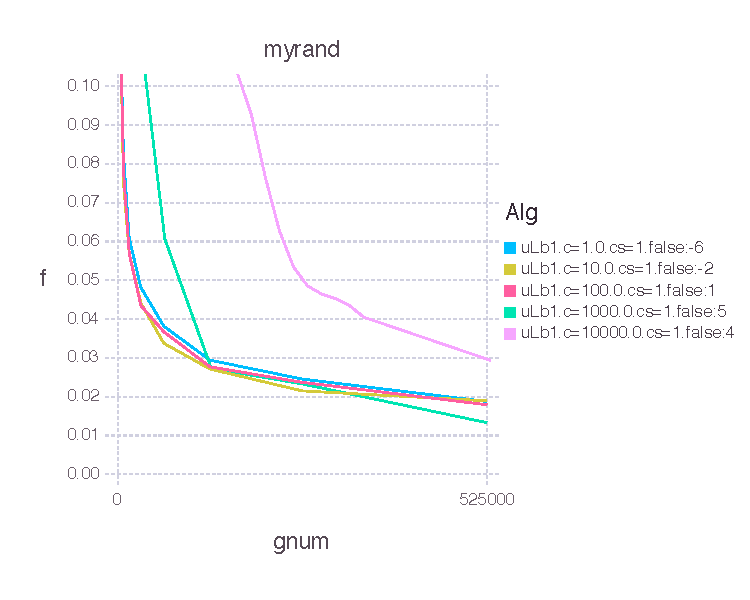
\includegraphics[width=\textwidth]{Figures/myrandBLtrueffFinal-linfalse.pdf}
              \caption{EGR-lin(SAG)}
          \end{subfigure}
          ~ %add desired spacing between images, e. g. ~, \quad, \qquad, \hfill etc. 
            %(or a blank line to force the subfigure onto a new line)
          \begin{subfigure}[b]{0.45\textwidth}
              \includegraphics[width=\textwidth]{Figures/myrandBLtrueffFinal-lintrue.pdf}
              \caption{EGR-lin(SAGA)} 
          \end{subfigure}
	   
   	    \begin{subfigure}[b]{0.45\textwidth}
              \includegraphics[width=\textwidth]{Figures/myrandBLtrueffFinal-quadfalse.pdf}
              \caption{EGR-quad(SAG)}
          \end{subfigure}
          ~ %add desired spacing between images, e. g. ~, \quad, \qquad, \hfill etc. 
            %(or a blank line to force the subfigure onto a new line)
          \begin{subfigure}[b]{0.45\textwidth}
              \includegraphics[width=\textwidth]{Figures/myrandBLtrueffFinal-quadtrue.pdf}
              \caption{EGR-quad(SAGA)}
          \end{subfigure}
	   
          \begin{subfigure}[b]{0.45\textwidth}
              \includegraphics[width=\textwidth]{Figures/myrandBLtrueffFinal-expfalse.pdf}
              \caption{EGR-exp(SAG)}
          \end{subfigure}
          ~ %add desired spacing between images, e. g. ~, \quad, \qquad, \hfill etc. 
            %(or a blank line to force the subfigure onto a new line)
            \begin{subfigure}[b]{0.45\textwidth}
                \includegraphics[width=\textwidth]{Figures/myrandBLtrueffFinal-exptrue.pdf}
                \caption{EGR-exp(SAGA)}
            \end{subfigure}
          \caption{myrand detailed: Comparing various growth rates. In the legend, $r$ is the parameter from Table \ref{tab1} and $a=log_2(\alpha)$ where $\alpha$ is the constant stepsize parameter.}\label{fig:myrand}
      \end{figure}
   
      \begin{figure}[H]
          \centering
   \begin{subfigure}[b]{0.45\textwidth}
              \includegraphics[width=\textwidth]{Figures/alphaGoodBLtrueffFinal-linfalse.pdf}
              \caption{EGR-lin(SAG)}
          \end{subfigure}
          ~ %add desired spacing between images, e. g. ~, \quad, \qquad, \hfill etc. 
            %(or a blank line to force the subfigure onto a new line)
          \begin{subfigure}[b]{0.45\textwidth}
              \includegraphics[width=\textwidth]{Figures/alphaGoodBLtrueffFinal-lintrue.pdf}
              \caption{EGR-lin(SAGA)} 
          \end{subfigure}
	   
   	    \begin{subfigure}[b]{0.45\textwidth}
              \includegraphics[width=\textwidth]{Figures/alphaGoodBLtrueffFinal-quadfalse.pdf}
              \caption{EGR-quad(SAG)}
          \end{subfigure}
          ~ %add desired spacing between images, e. g. ~, \quad, \qquad, \hfill etc. 
            %(or a blank line to force the subfigure onto a new line)
          \begin{subfigure}[b]{0.45\textwidth}
              \includegraphics[width=\textwidth]{Figures/alphaGoodBLtrueffFinal-quadtrue.pdf}
              \caption{EGR-quad(SAGA)}
          \end{subfigure}
	   
          \begin{subfigure}[b]{0.45\textwidth}
              \includegraphics[width=\textwidth]{Figures/alphaGoodBLtrueffFinal-expfalse.pdf}
              \caption{EGR-exp(SAG)}
          \end{subfigure}
          ~ %add desired spacing between images, e. g. ~, \quad, \qquad, \hfill etc. 
            %(or a blank line to force the subfigure onto a new line)
            \begin{subfigure}[b]{0.45\textwidth}
                \includegraphics[width=\textwidth]{Figures/alphaGoodBLtrueffFinal-exptrue.pdf}
                \caption{EGR-exp(SAGA)}
            \end{subfigure}
          \caption{alphaGood detailed: Comparing various growth rates. In the legend, $r$ is the parameter from Table \ref{tab1} and $a=log_2(\alpha)$ where $\alpha$ is the constant stepsize parameter.}\label{fig:alphaGood}
      \end{figure}
   
      \begin{figure}[H]
          \centering
   \begin{subfigure}[b]{0.45\textwidth}
              \includegraphics[width=\textwidth]{Figures/SUSYBLtrueffFinal-linfalse.pdf}
              \caption{EGR-lin(SAG)}
          \end{subfigure}
          ~ %add desired spacing between images, e. g. ~, \quad, \qquad, \hfill etc. 
            %(or a blank line to force the subfigure onto a new line)
          \begin{subfigure}[b]{0.45\textwidth}
              \includegraphics[width=\textwidth]{Figures/SUSYBLtrueffFinal-lintrue.pdf}
              \caption{EGR-lin(SAGA)} 
          \end{subfigure}
	   
   	    \begin{subfigure}[b]{0.45\textwidth}
              \includegraphics[width=\textwidth]{Figures/SUSYBLtrueffFinal-quadfalse.pdf}
              \caption{EGR-quad(SAG)}
          \end{subfigure}
          ~ %add desired spacing between images, e. g. ~, \quad, \qquad, \hfill etc. 
            %(or a blank line to force the subfigure onto a new line)
          \begin{subfigure}[b]{0.45\textwidth}
              \includegraphics[width=\textwidth]{Figures/SUSYBLtrueffFinal-quadtrue.pdf}
              \caption{EGR-quad(SAGA)}
          \end{subfigure}
	   
          \begin{subfigure}[b]{0.45\textwidth}
              \includegraphics[width=\textwidth]{Figures/SUSYBLtrueffFinal-expfalse.pdf}
              \caption{EGR-exp(SAG)}
          \end{subfigure}
          ~ %add desired spacing between images, e. g. ~, \quad, \qquad, \hfill etc. 
            %(or a blank line to force the subfigure onto a new line)
            \begin{subfigure}[b]{0.45\textwidth}
                \includegraphics[width=\textwidth]{Figures/SUSYBLtrueffFinal-exptrue.pdf}
                \caption{EGR-exp(SAGA)}
            \end{subfigure}
          \caption{SUSY detailed: Comparing various growth rates. In the legend, $r$ is the parameter from Table \ref{tab1} and $a=log_2(\alpha)$ where $\alpha$ is the constant stepsize parameter.}\label{fig:SUSY}
      \end{figure}
   

      \begin{figure}[H]
          \centering
          \begin{subfigure}[b]{0.45\textwidth}
              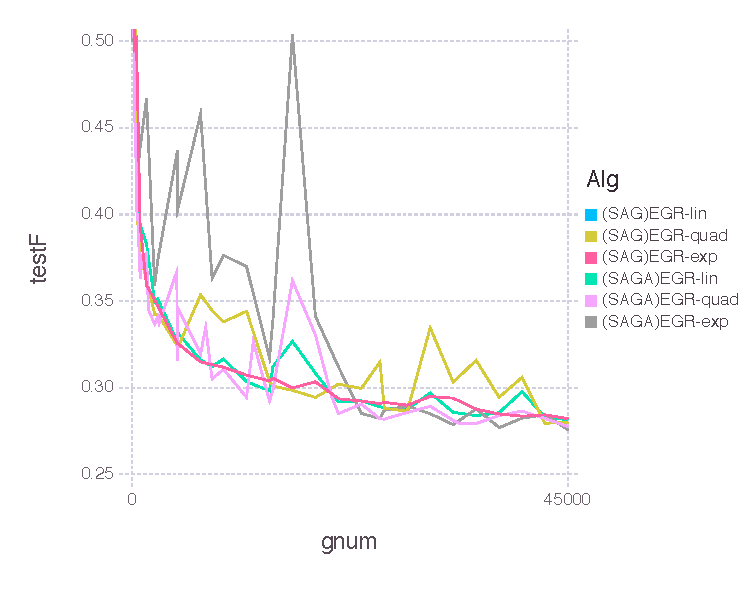
\includegraphics[width=\textwidth]{Figures/MNISTBLtrueFfFinal-1.pdf}
              \caption{Current F value}
          \end{subfigure}
          ~ %add desired spacing between images, e. g. ~, \quad, \qquad, \hfill etc. 
            %(or a blank line to force the subfigure onto a new line)
            \begin{subfigure}[b]{0.45\textwidth}
                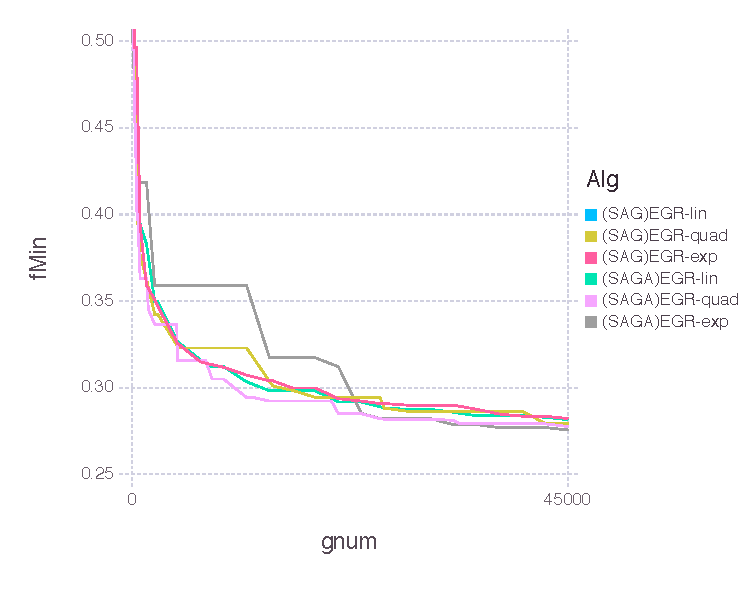
\includegraphics[width=\textwidth]{Figures/MNISTBLtrueFminfFinal-2.pdf}
                \caption{Incumbent best solution}
            \end{subfigure}
          \caption{MNIST summary: all EGR methods}\label{fig:MNISTsummary}
      \end{figure}
   
   

   \begin{figure}[H]
       \centering
       \begin{subfigure}[b]{0.45\textwidth}
           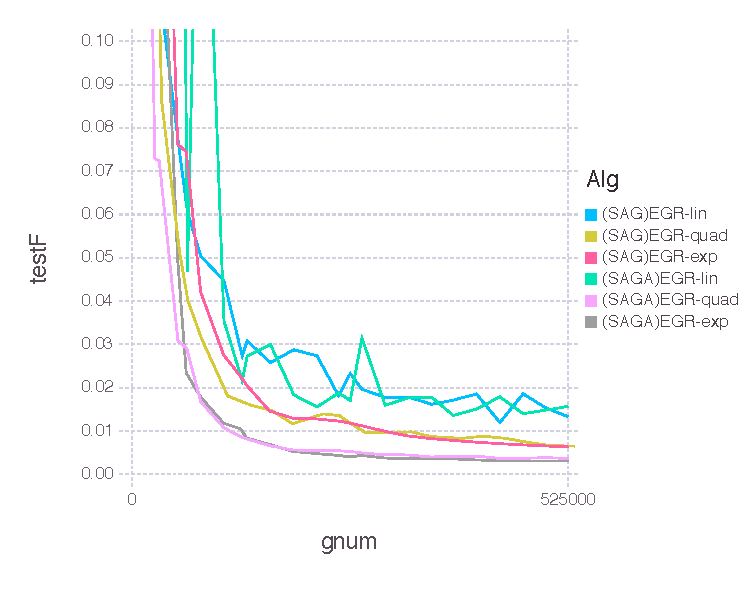
\includegraphics[width=\textwidth]{Figures/myrandBLtrueFfFinal-1.pdf}
           \caption{Current F value}
       \end{subfigure}
       ~ %add desired spacing between images, e. g. ~, \quad, \qquad, \hfill etc. 
         %(or a blank line to force the subfigure onto a new line)
         \begin{subfigure}[b]{0.45\textwidth}
             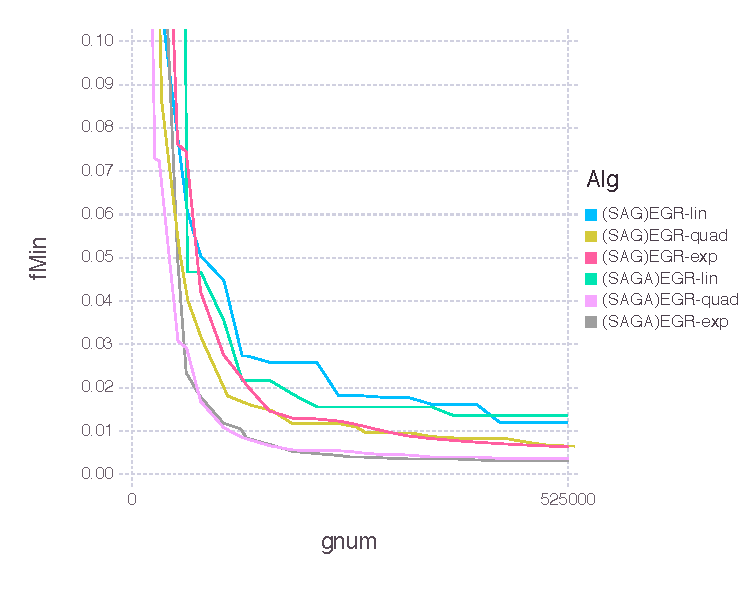
\includegraphics[width=\textwidth]{Figures/myrandBLtrueFminfFinal-2.pdf}
             \caption{Incumbent best solution}
         \end{subfigure}
       \caption{myrand summary: all EGR methods}\label{fig:myrandsummary}
   \end{figure}
   %
   \begin{figure}[H]
       \centering
       \begin{subfigure}[b]{0.45\textwidth}
           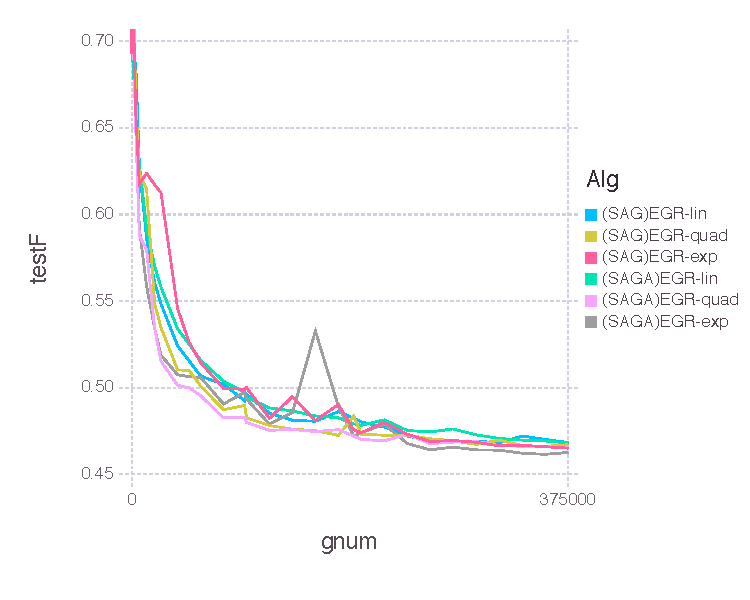
\includegraphics[width=\textwidth]{Figures/alphaGoodBLtrueFfFinal-1.pdf}
           \caption{Current F value}
       \end{subfigure}
       ~ %add desired spacing between images, e. g. ~, \quad, \qquad, \hfill etc.
         %(or a blank line to force the subfigure onto a new line)
         \begin{subfigure}[b]{0.45\textwidth}
             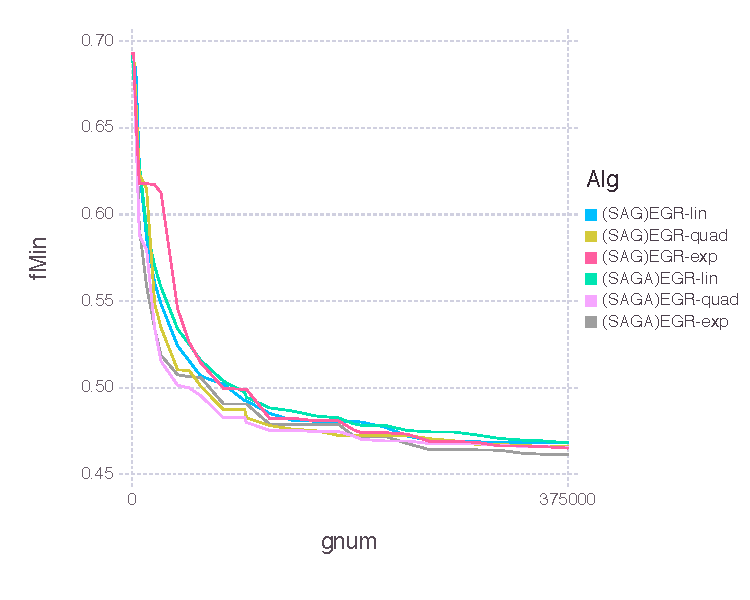
\includegraphics[width=\textwidth]{Figures/alphaGoodBLtrueFminfFinal-2.pdf}
             \caption{Incumbent best solution}
         \end{subfigure}
       \caption{alphaGood summary: all EGR methods}\label{fig:alphaGoodsummary}
   \end{figure}

   \begin{figure}[H]
       \centering
       \begin{subfigure}[b]{0.45\textwidth}
           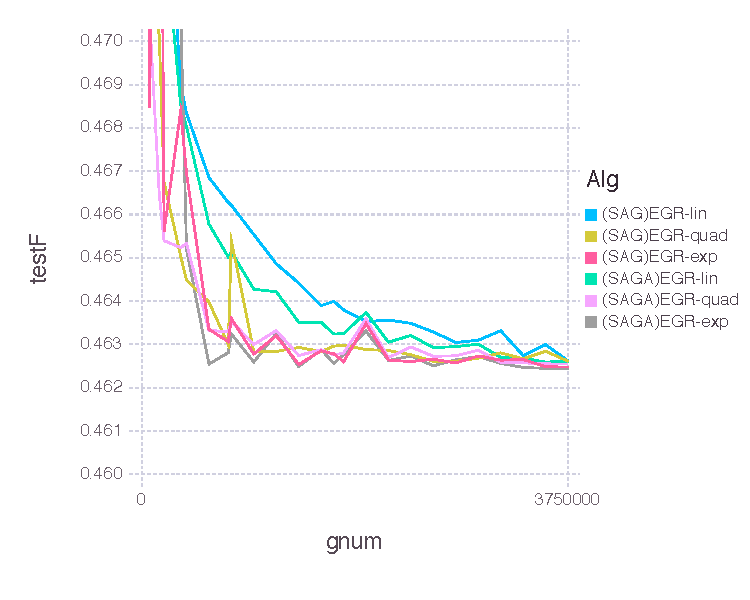
\includegraphics[width=\textwidth]{Figures/SUSYBLtrueFfFinal-1.pdf}
           \caption{Current F value}
       \end{subfigure}
       ~ %add desired spacing between images, e. g. ~, \quad, \qquad, \hfill etc.
         %(or a blank line to force the subfigure onto a new line)
         \begin{subfigure}[b]{0.45\textwidth}
             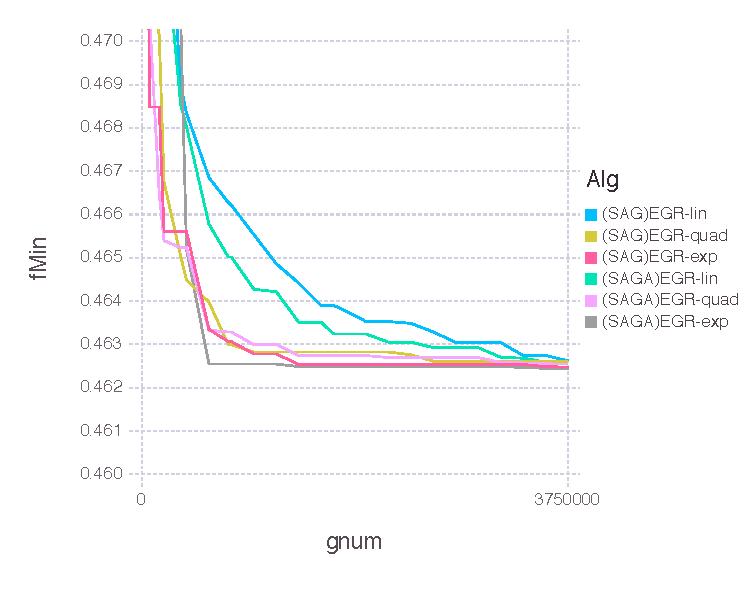
\includegraphics[width=\textwidth]{Figures/SUSYBLtrueFminfFinal-2.pdf}
             \caption{Incumbent best solution}
         \end{subfigure}
       \caption{SUSY summary: all EGR methods}\label{fig:SUSYsummary}
   \end{figure}
   
   
		 
   On problem MNIST, in Figure \ref{fig:MNIST}, we see that for linear EGR-SAGA, smaller batch sizes are preferable. When $r=1$, the method performs extremely well, but slightly increasing the batch to $r=10$ allows for significantly larger stepsizes to be taken. This closely resembles the common knowlegde about the need for mini-batching in SG methods. As r increases, larger steplengths are needed for good performance: this is logical since the methods use more new informantion at each iteration, thus having less variance in the step directions. Large batch sizes do not work well, since the method only takes a few iterations. For the linear EGR-SAG, the additional stability introduced by the slightly increased batch size ($r=10$) is more pronounced.  For quadratic EGR-SAGA, the smallest $r$ tested gives the same method as the linear $r=1$ method because of rounding. Improved performance for slightly higher $r$ values can be attributed to the additional stability stemming from increasing batch sizes in the later iterations. For quadratic EGR-SAG, while increasing beyond $r=1e-5$ does not seem to benefit the final objective value achieved, the stability of the method is apparent. The the exponentially growing case, the same idea as before applies: A slightly increasing batch size in the latter iterations seems to benefit the stability and sometimes the performance of the methods. Value of $r=1,000$ seems to perform well. 
   
   In Figure~\ref{fig:MNISTsummary}, we combine these methods in a single plot. The EGR-SAGA methods with growing batch sizes at the end seem to work best in practice. We attribute this to the unbiased nature of the methods. In both cases, we see that it is beneficial to increase the batches at the end, instead of leaving them 1 and 1 constantly. 

   
   
   With the myrand dataset, the picture is slightly different. In Figure~\ref{fig:myrand}, we can clearly see that the relative growth rates are higher than for MNIST, and the take-off points occur earlier than in MNIST. In Figure~\ref{fig:myrandsummary}, we again see the clear advantage of using growing batch sizes, but in this case the growth rates are higher than in MNIST.
    
  
  We do not claim to have exhastively searched all possible growth rates. Rather, we presented three reasonable choices, with one having a strong theoretical support. On some problems, an alternative growth rate works well: Starting with a large initial batch
   \subsubsection{Only Add Comparison}
   
   The only-add option in EGR includes many existing methods, such as SG and DSS. We empirically compare the performance of our new methods with SG and DSS.
   The Stochastic Gradient method enjoys immense popularity in both the optimization and the machine learning communities, and when carefully tuned can outperform any known modern method. The tuning often involves intricate step size strategies. We do not attempt to compare with the best SG implementation, rather we demonstrate the benefits of using the EGR scheme, compared to SG, with both methods using a constant step size. 
   
   
   

   \begin{figure}[H]
       \centering
       \begin{subfigure}[b]{0.45\textwidth}
           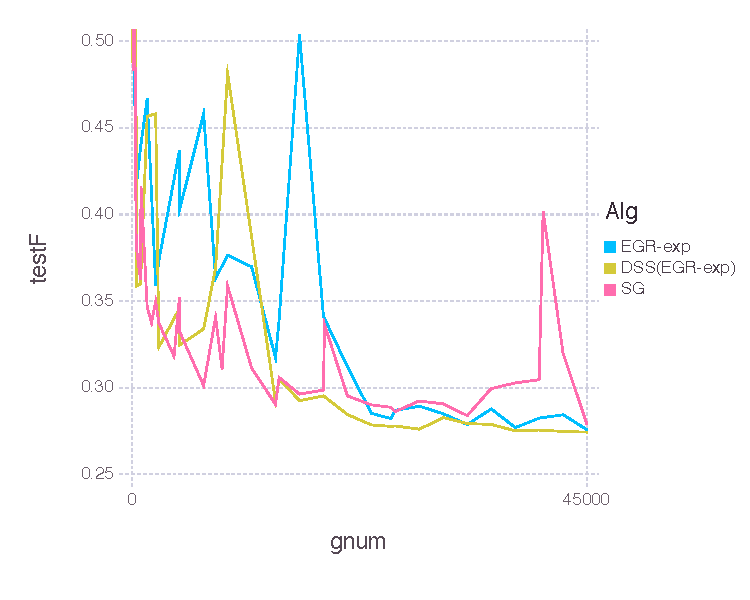
\includegraphics[width=\textwidth]{Figures/MNISTBLtrueFfFinal-dss.pdf}
           \caption{Current F value}
       \end{subfigure}
       ~ %add desired spacing between images, e. g. ~, \quad, \qquad, \hfill etc.
         %(or a blank line to force the subfigure onto a new line)
         \begin{subfigure}[b]{0.45\textwidth}
             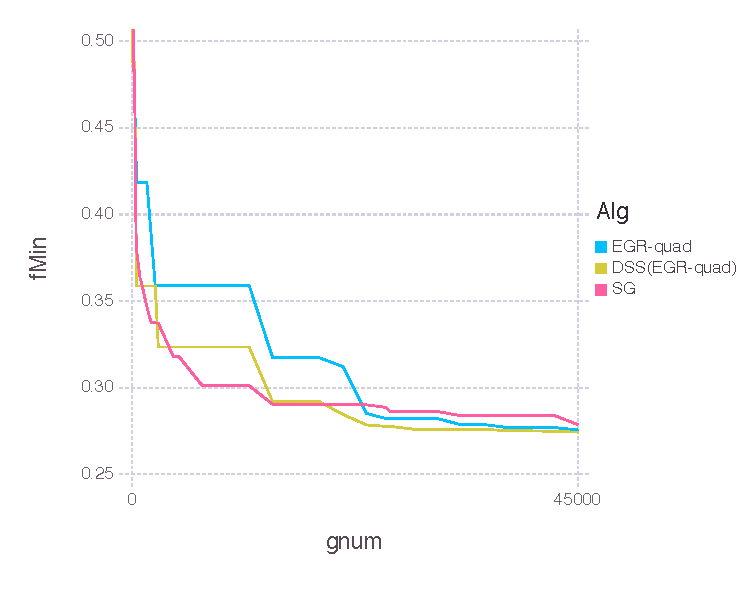
\includegraphics[width=\textwidth]{Figures/MNISTBLtrueFminfFinal-dss.pdf}
             \caption{Incumbent best solution}
         \end{subfigure}
       \caption{MNIST: EGR vs only-add methods}\label{fig:MNISToa}
   \end{figure}
   
   \begin{figure}[H]
       \centering
       \begin{subfigure}[b]{0.45\textwidth}
           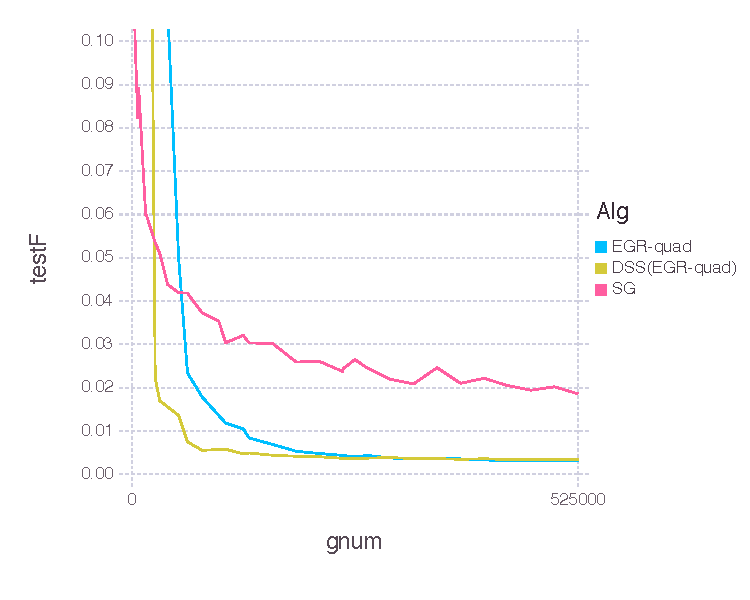
\includegraphics[width=\textwidth]{Figures/myrandBLtrueFfFinal-dss.pdf}
           \caption{Current F value}
       \end{subfigure}
       ~ %add desired spacing between images, e. g. ~, \quad, \qquad, \hfill etc.
         %(or a blank line to force the subfigure onto a new line)
         \begin{subfigure}[b]{0.45\textwidth}
             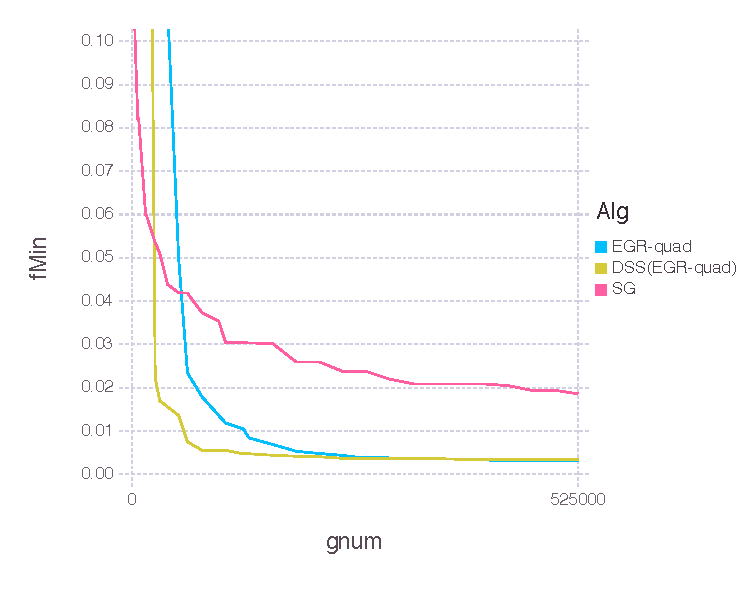
\includegraphics[width=\textwidth]{Figures/myrandBLtrueFminfFinal-dss.pdf}
             \caption{Incumbent best solution}
         \end{subfigure}
       \caption{myrand: EGR vs only-add methods}\label{fig:myrandoa}
   \end{figure}
   
   \begin{figure}[H]
       \centering
       \begin{subfigure}[b]{0.45\textwidth}
           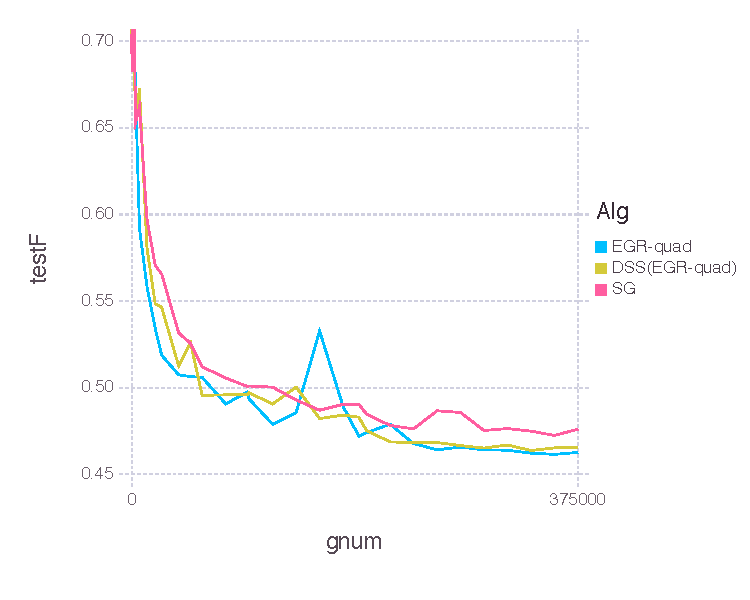
\includegraphics[width=\textwidth]{Figures/alphaGoodBLtrueFfFinal-dss.pdf}
           \caption{Current F value}
       \end{subfigure}
       ~ %add desired spacing between images, e. g. ~, \quad, \qquad, \hfill etc.
         %(or a blank line to force the subfigure onto a new line)
         \begin{subfigure}[b]{0.45\textwidth}
             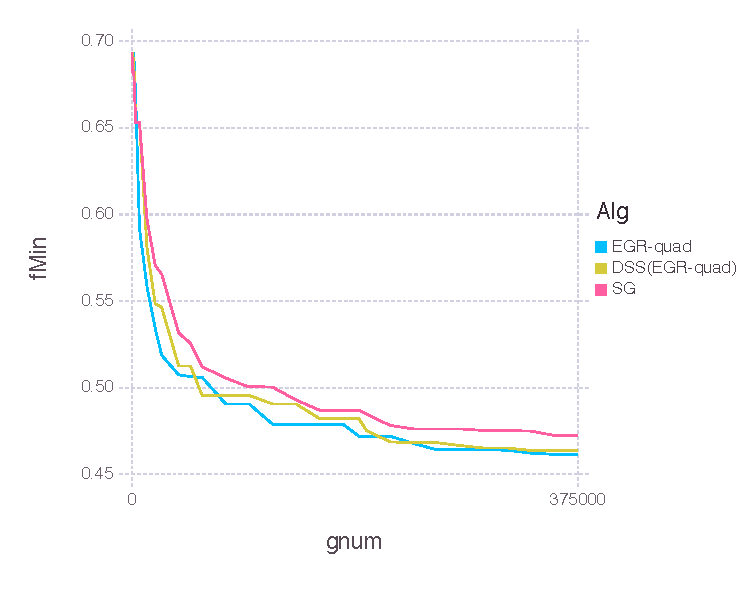
\includegraphics[width=\textwidth]{Figures/alphaGoodBLtrueFminfFinal-dss.pdf}
             \caption{Incumbent best solution}
         \end{subfigure}
       \caption{alphaGood: EGR vs only-add methods}\label{fig:alphaGoodoa}
   \end{figure}
   
   \begin{figure}[H]
       \centering
       \begin{subfigure}[b]{0.45\textwidth}
           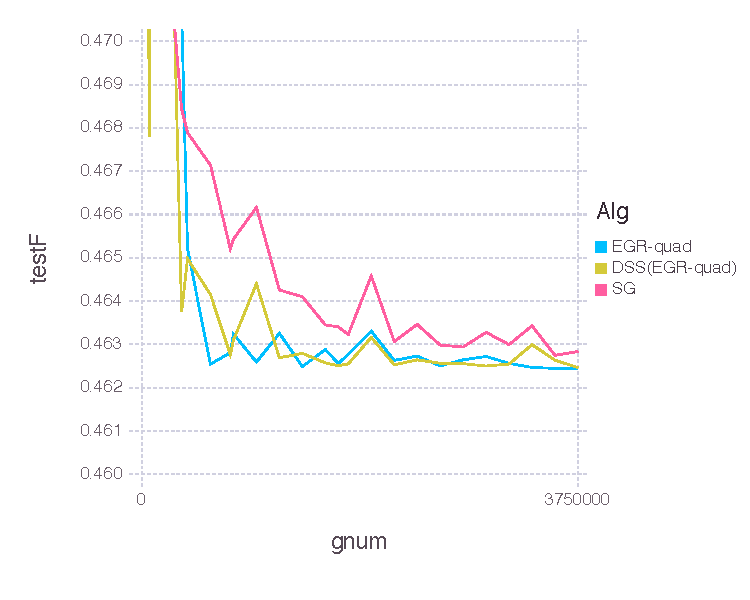
\includegraphics[width=\textwidth]{Figures/SUSYBLtrueFfFinal-dss.pdf}
           \caption{Current F value}
       \end{subfigure}
       ~ %add desired spacing between images, e. g. ~, \quad, \qquad, \hfill etc.
         %(or a blank line to force the subfigure onto a new line)
         \begin{subfigure}[b]{0.45\textwidth}
             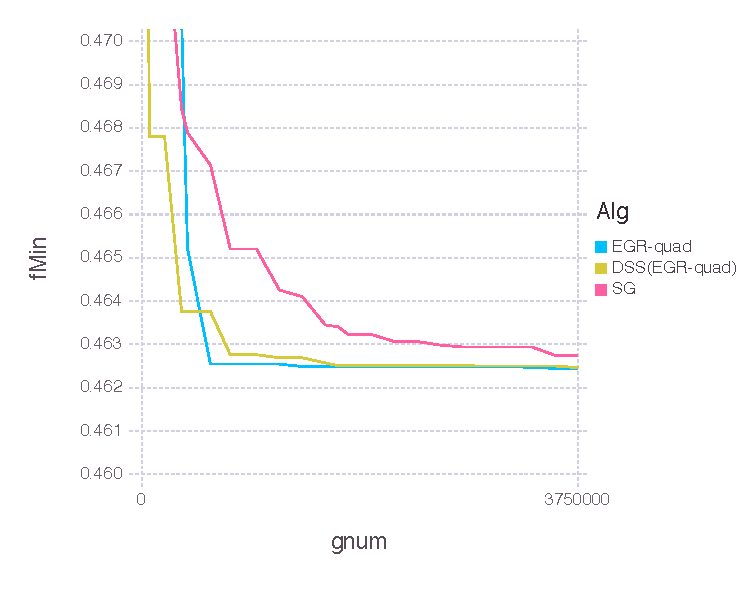
\includegraphics[width=\textwidth]{Figures/SUSYBLtrueFminfFinal-dss.pdf}
             \caption{Incumbent best solution}
         \end{subfigure}
       \caption{SUSY: EGR vs only-add methods}\label{fig:SUSYoa}
   \end{figure}
   
   
   \subsubsection{Performance Comparison}   
    
   We compare the EGR method with other... FINITO seems to be an appropriate method to compare with, since a precise streaming version of the algorithm is presented in the original paper. S-SVRG, while being seemingly a perfect fit for our objective was not competitive on any test problem. 
   
   The SAGinit and SAGAinit methods are not commonly thought of as optimization methods, but are presented as initialization heuristics in the corresponding papers. Nevertheless, the methods are considered as a way to run these aggregated gradient methods while buliding up memory as you go along. For example, the SAGinit method presented in \cite{roux2012stochastic}, can be written as follows:
   
   Note the major differences with the EGR framework: The decision to update a previously sampled point or to sample a new function is a random variable, as opposed to pre-defined sequences $s_k$ and $u_k$ in EGR. 

   \begin{figure}[H]
       \centering
       \begin{subfigure}[b]{0.45\textwidth}
           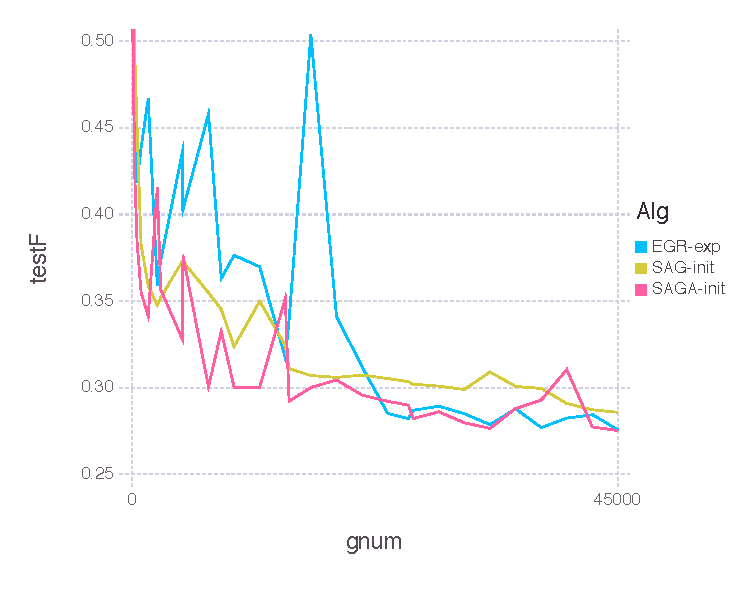
\includegraphics[width=\textwidth]{Figures/MNISTBLtrueFfFinal-g.pdf}
           \caption{Current F value}
       \end{subfigure}
       ~ %add desired spacing between images, e. g. ~, \quad, \qquad, \hfill etc.
         %(or a blank line to force the subfigure onto a new line)
         \begin{subfigure}[b]{0.45\textwidth}
             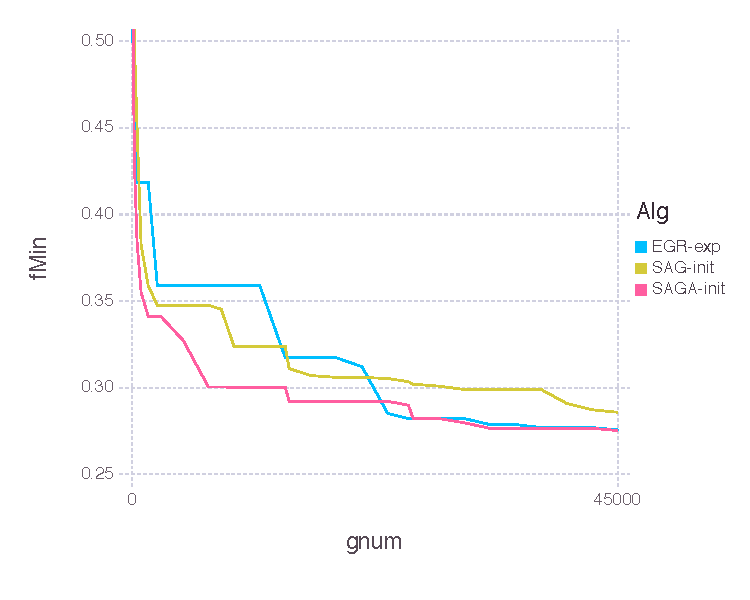
\includegraphics[width=\textwidth]{Figures/MNISTBLtrueFminfFinal-g.pdf}
             \caption{Incumbent best solution}
         \end{subfigure}
       \caption{MNIST: EGR vs other methods}\label{fig:MNISTom}
   \end{figure}
   
   \begin{figure}[H]
       \centering
       \begin{subfigure}[b]{0.45\textwidth}
           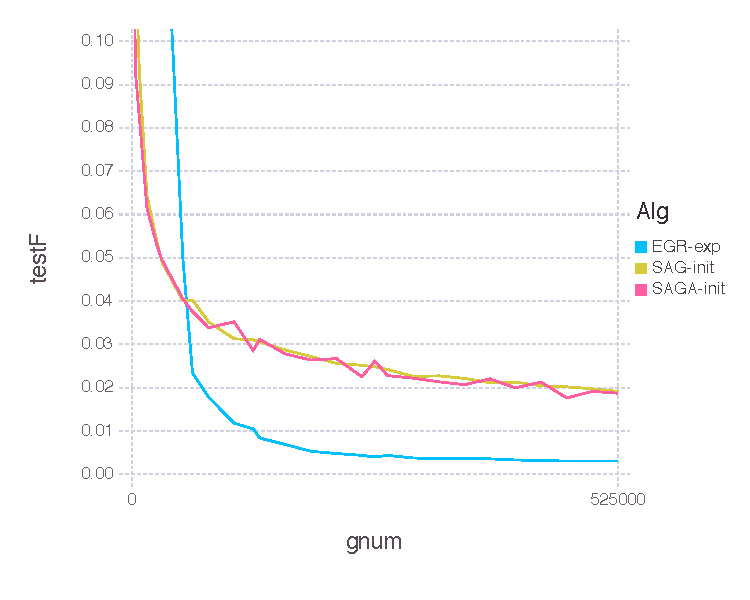
\includegraphics[width=\textwidth]{Figures/myrandBLtrueFfFinal-g.pdf}
           \caption{Current F value}
       \end{subfigure}
       ~ %add desired spacing between images, e. g. ~, \quad, \qquad, \hfill etc.
         %(or a blank line to force the subfigure onto a new line)
         \begin{subfigure}[b]{0.45\textwidth}
             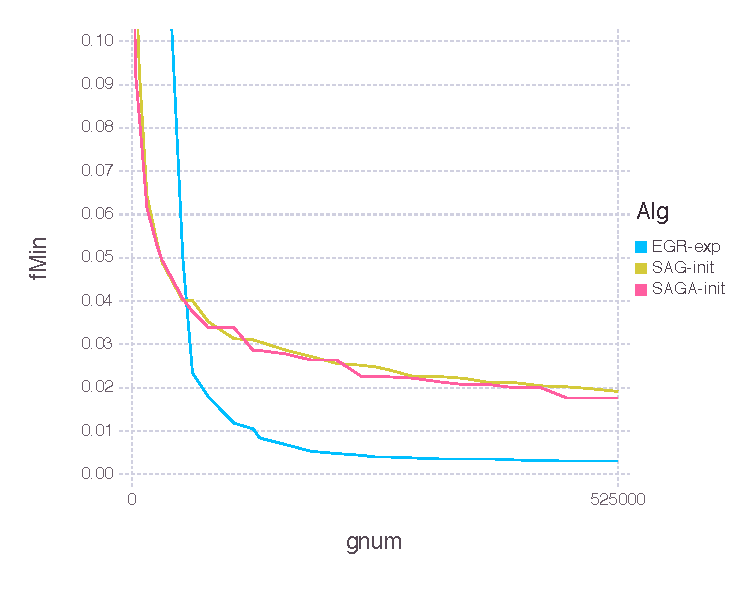
\includegraphics[width=\textwidth]{Figures/myrandBLtrueFminfFinal-g.pdf}
             \caption{Incumbent best solution}
         \end{subfigure}
       \caption{myrand: EGR vs other methods}\label{fig:myrandom}
   \end{figure}
   
   \begin{figure}[H]
       \centering
       \begin{subfigure}[b]{0.45\textwidth}
           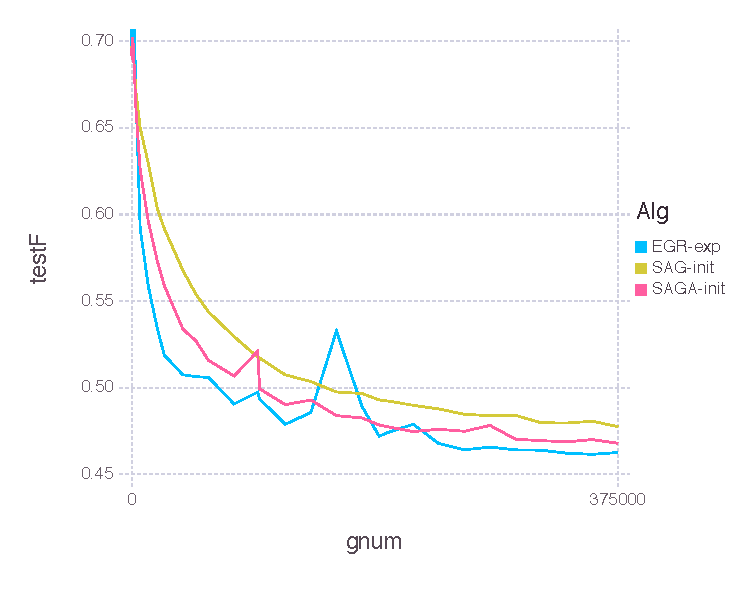
\includegraphics[width=\textwidth]{Figures/alphaGoodBLtrueFfFinal-g.pdf}
           \caption{Current F value}
       \end{subfigure}
       ~ %add desired spacing between images, e. g. ~, \quad, \qquad, \hfill etc.
         %(or a blank line to force the subfigure onto a new line)
         \begin{subfigure}[b]{0.45\textwidth}
             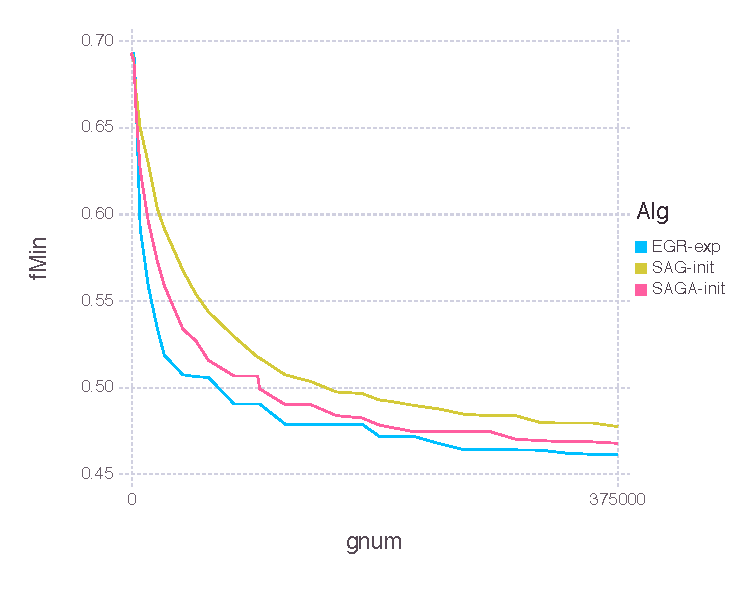
\includegraphics[width=\textwidth]{Figures/alphaGoodBLtrueFminfFinal-g.pdf}
             \caption{Incumbent best solution}
         \end{subfigure}
       \caption{alphaGood: EGR vs other methods}\label{fig:alphaGoodom}
   \end{figure}
   
   \begin{figure}[H]
       \centering
       \begin{subfigure}[b]{0.45\textwidth}
           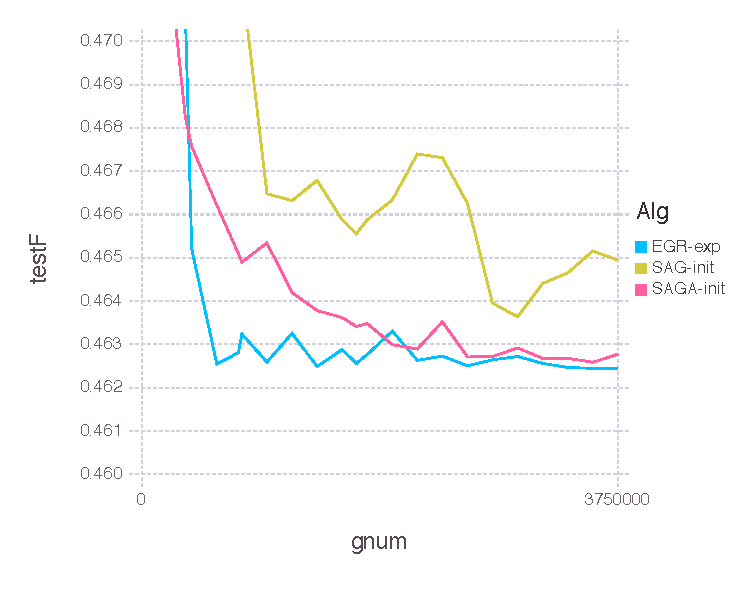
\includegraphics[width=\textwidth]{Figures/SUSYBLtrueFfFinal-g.pdf}
           \caption{Current F value}
       \end{subfigure}
       ~ %add desired spacing between images, e. g. ~, \quad, \qquad, \hfill etc.
         %(or a blank line to force the subfigure onto a new line)
         \begin{subfigure}[b]{0.45\textwidth}
             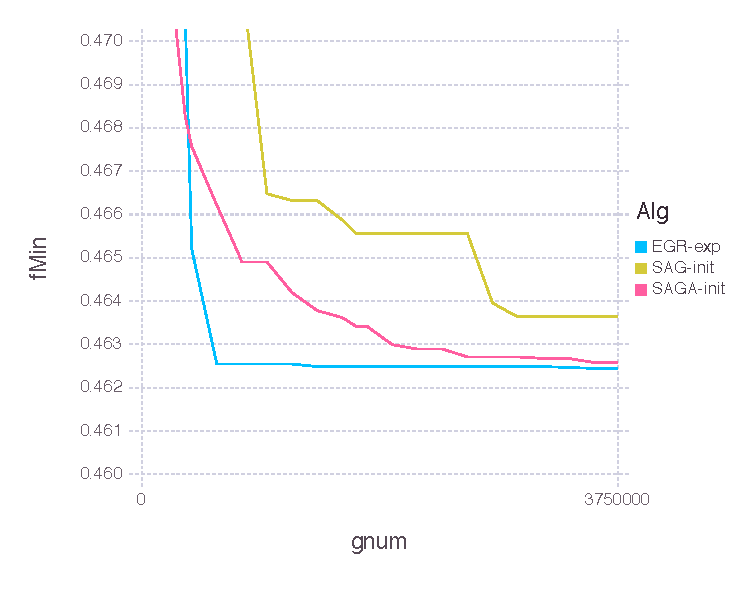
\includegraphics[width=\textwidth]{Figures/SUSYBLtrueFminfFinal-g.pdf}
             \caption{Incumbent best solution}
         \end{subfigure}
       \caption{SUSY: EGR vs other methods}\label{fig:SUSYom}
   \end{figure}
   
   \subsubsection{Memory Reduction Techniques in Practice}
   
   The following experiments show the algorithm progress after 40 passes over the data. Only two types of chunking are tested: SAG and SAGA chunking. The labels are in the format \texttt{algorithm numChunks StepsizePower}. The stepsizes were tuned to give the best final function value. 
   
   The follwing experiements show comparisons of the aggregated gradient methods SAG and SAGA with respect to Batching vs Chunking. We conducted experiments comparing Chunking vs Batching on three datasets, and two aggregated gradient methods: SAG and SAGA. This experiment was suggested to verify the previous chunking results (on pages 41-43), because these previous experiments suggested that the chunking idea is not working well in practice. 

   The new experiments are ran with 40 equivalent passes over the data, and stepsizes were chosen to give the best possible function value over the progress of all iterations. Each method was tested with the following two configurations:
   a) Batching - batches of size 2, chunks of size 1  (blue and red on plots)
   b) Chunking - chunks of size 2, batches of size 1 (yellow and green on plots)

   The chunking methods seem to perform much worse than the equivalent batching methods.

\section{Final Remarks} \label{finalr}


 \small 
\bibliographystyle{plain}

\bibliography{../References/references}


\end{document}
